\chapter{Grammar}

To begin with I would like to say that grammar is the core of every language. Grammar comprises different themes that are united in a system of changing words enough for building sensible syntax constructions. We will look at Novoslovnica grammar from the point of Parts of Speech.

Part of speech (POS) - is a category of words which have similar grammatical properties.

Thus we unite some words into parts of speech when there are a lot of similar grammar properties, such as “number”, “person”, “case”, “tense” etc. In this chapter we will go through different parts of speech and study what differences they have and how we should deal with them. 

POS have two main categories - independent parts of speech and auxiliary parts of speech. Why some of POS are auxiliary or independent? This refers to their semantic values. Independent POS have a full semantic value. Auxiliary have not. What it means: when you say a word of an independent POS you reproduce some meaning that the interlocutor can recognize.

\textbf{Example:}

\textit{River} - this word can be recognized by interlocutor as some concept of water flowing in a restricted area.

\textit{Beautiful} - this word is recognizable as an attribute of any concept that is nice, pleasant to the person (i.e. speaker or interlocutor)

\textit{Came} - this word can be recognized as any concept’s action of going to the destination point and having reached it. 

And so on. You see that every word has its own meaning, rather full to imagine yourself some information you have been received. This is not true for auxiliary POS. For example, words “and” or “to” cannot give you any map in your mind into any sensible meanings. Though these words have no determined sense itselves, they are extremely important in the whole phrase. English language is an analytical one, that’s why words are mostly connected with each other in the phrase by auxiliary POS. Without them you cannot understand, what the person have said to you. Slavic languages are fusional, but there are enough analytic features in them, hence auxiliary POS are also important.

Also there are two additional categories - particles and interjections. Some allocate them into separate categories, some claim they belong to an auxiliary category. Nevertheless, these are separated POS that have different properties.

Particles add to words they are close to some additional functions. If you delete them from your phrase, there will be no change in the whole meaning (that’s why I cannot say they are an auxiliary ones), but with presence of particles you will get more semantic or emotional information. English language has very few particles. The most known is “to” as an infinitive indicator particle of a verb. Controversially, Slavic languages have a bit more particles, that are rather popular in the spoken language. 

\textbf{Examples:}

\textit{Ja sům govoril tobě. }- I have told you.

\textit{Ja sům govoril že tobě!} - I have told you! (Additional semantic meaning. The speaker shifts emphasis from undefined to the word “govoril” (told). So the interlocutor now have a determined emphasis of the phrase. The speaker wants to say that he has already told the same fact to the interlocutor and his idea has become true just now.) 

Interjection is a POS that have no semantic meanings. They are not words in over common comprehension. Interjections are sounds that we produce. It is rather difficult to say sometimes what differences are between interjections and senseless sounds that we can produce (i.e. some spontaneous exclaims, murmuring etc.) Interjections are divided into intended exclaims (with bright emotional color) and sound imitations (i.e. animal voices imitation).

These are categories of POS. If we speak about independent POS, we should take into account that there are different semantic, morphological and syntax functions can be described by these POS. There several type of these functions: the concept, the attribute, the predicate and the demonstrative.

The concept is something that correlates with the object or subject in the real world. It could be either abstract or imaginary, but we can ask a questions “Who? What?” about it.

The predicate is something that determines the action, corresponding to a concept. We often ask questions “What to do?” to reveal a predicate.

The attribute is something that is correspond to a concept or an action. We ask questions “What concept is like?” or “What action is like?” to find out the determine value of the attribute.

The demonstrative points out the concept. It has the same question with the attribute, yet has no semantic value but demonstrating a concept it corresponds with. 

POS with concept properties are Nouns and Cardinal Numerals. POS with attribute properties are Adjectives. Ordinal Numerals and Adverbs. POS with action properties are Verbs, Participles, Gerund. POS with demonstrative attributes are Pronouns.

Thus Noun, Adjective, Verb, Adverb, Numeral, Pronoun, Gerund, Participle are independent while Preposition, Particle, Interjection, Conjunction are auxiliary.

The last division of independent POS is nominal/verbal. It is extremely important, because this division shows differences in grammar of nominal and verbal POS. Verb, Participle, Gerund are verbal POS while Noun, Adjective, Numeral are nominal. Adverbs and pronouns stay separately - the first one because of its immutability and the second one because of its heterogeneity. 

In this chapter we will speak about every POS I have listed above. In the beginning of each paragraph I will give you a table of some kind of property description of the POS.

First you should know some facts about different grammatical properties in Novoslovnica.


\newcounter{casechapter}[section]
\section{Case}

Case\index{case} is a grammatical property of a nominal POS (Part of speech) that shows what references this nominal POS has with other words in a sentence (phrase). This property is widely known in fusional languages, while analytical languages do not often possess this property. Thus, English has only two active cases - Nominative and Oblique one. Moreover, oblique case is used practically only within pronouns while nouns have no such a case. That means case is not the only way to show references between nominal POS and other words in a sentence. Case is just one of the ways to show it and Slavic languages as being fusional widely use this grammar category.

Different Slavic languages have different number of cases. For example, Russian language has six cases while Serbian language has seven. We can find exceptions in Bulgarian and Macedonian languages, which are analytical that is why they have only one case for a noun and adjective and three cases for a pronoun.

Different cases are referred to different semantic links between words. It is the cause why we see ambiguity of cases in different languages (that have different amount of cases and different usage rules of cases). Novoslovnica provides most common and wide means to use cases with almost full determination. When you speak Novoslovnica you have to use the case of exact semantic value and not of the longstanding phraseology of your own language.

With this principle Novoslovnica establishes nine cases. Nine changing patterns that determine alterations of all words of nominal POS. This is the unification of Slavic languages in the sphrere of fusial word linking. Here they are:

\newglossaryentry{nominative}{name=P.C., description={Nominative}}
\newglossaryentry{genitive}{name=G.C., description={Genitive}}
\newglossaryentry{partitive}{name=P.C., description={Partitive}}
\newglossaryentry{accusative}{name=A.C., description={Accusative}}
\newglossaryentry{dative}{name=D.C., description={Dative}}
\newglossaryentry{instrumental}{name=I.C., description={Instrumental}}
\newglossaryentry{prepositional}{name=Pr.C., description={Prepositional}}
\newglossaryentry{locative}{name=L.C., description={Locative}}
\newglossaryentry{vocative}{name=V.C., description={Vocative}}

\begin{itemize}
	\item Nominative (\gls{nominative})
	\item Genitive (\gls{genitive})
	\item Partitive (\gls{partitive})
	\item Dative (\gls{dative})
	\item Accusative (\gls{accusative})
	\item Instrumental (\gls{instrumental})
	\item Prepositional (\gls{prepositional})
	\item Locative (\gls{locative})
	\item Vocative (\gls{vocative})
\end{itemize}

In this chapter we will speak about cases in general. All examples will disclose case features through nouns as examples.

Nominative\index{case!nominative} case (\textit{Imenóvnik}) is used when we are talking about a concept as an actor. If the sentence is full, the subject is in Nominative. You can ask questions like «Who? What?» to it.

This case is basic in most languages, so POSes in this case are supposed to be in the normal form (that we can find in a dictionary). In Novoslovnica nominative also determines a normal from of the word. In the examples you can see full sentenses, where subject is used in nominative.

\textbf{Examples:}

\stepcounter{casechapter}
\arabic{chapter}.\arabic{section}.\arabic{casechapter} \textit{\textbf{Dom}-òt je vëlïkym.} - The \textbf{house} is big.

\stepcounter{casechapter}
\arabic{chapter}.\arabic{section}.\arabic{casechapter} \textit{\textbf{Izučilišto}, de ja sę učam, je starym}. - The \textbf{school} I attend is old.

\stepcounter{casechapter}
\arabic{chapter}.\arabic{section}.\arabic{casechapter} \textit{Klüč-òt je od ovoŭ vråtoŭ.} - The key is to these doors.

Genitive\index{case!genitive} case (\textit{Čyǐnik}) is used when we are talking to an object being related to another one. Thus this case show what generation the object is of and what is it made from or whom does it belong to. The questions that determine the case are «Whose? Which? What?».

In Novoslovnica possessive case equals to genitive one, so English «'s» constructions should be translated in genitive (example 4.1.4). Further, genitive in Novoslovnica could be related to usage of nouns with «of» preposition (example 2, 3).

\textbf{Examples:}

\stepcounter{casechapter}
\arabic{chapter}.\arabic{section}.\arabic{casechapter} \textit{Kniga \textbf{brata} je vëlïmi zajimliva.} — My \textbf{brother}'s book is very fascinating.

\stepcounter{casechapter}
\arabic{chapter}.\arabic{section}.\arabic{casechapter} \textit{Cěna \textbf{uspěha} je mnogo vëlïka.} — The price of \textbf{success} is very high.

\stepcounter{casechapter}
\arabic{chapter}.\arabic{section}.\arabic{casechapter} \textit{Sklad je na koncu \textbf{ulicy}-ta.} — The shop is at the end of the \textbf{street}.

Partitive\index{case!partitive} case (\textit{Ličóvnik}) is used when we are talking about some amount of object having or being supposed to have uncountable properties. The questions that determine the case are «Of what? With what? How much of?».

This case has many coinciding forms with genitive, though in masculine gender it has another endings (examples 1, 3). In English it should be translated with «of» construction (example 1). If uncountable nouns are used with the predicate directly or with adverbs of measure, they should be translated into Oblique case in English (example 2, 3).

\textbf{Examples:}

\stepcounter{casechapter}
\arabic{chapter}.\arabic{section}.\arabic{casechapter} \textit{Daǐ mi čašku \textbf{čaju}.} — Give me a cup of \textbf{tea}.

\stepcounter{casechapter}
\arabic{chapter}.\arabic{section}.\arabic{casechapter} \textit{Dodaǐ do pïroga němnogo \textbf{vody}.} — Add some \textbf{water} to a cake.

\stepcounter{casechapter}
\arabic{chapter}.\arabic{section}.\arabic{casechapter} \textit{Predaǐ mi \textbf{cukru}.} — Pass me \textbf{sugar}.

Dative case (\textit{Datelnik}) is used when we are talking about a noun to which something is given. We can ask a question for a word in this case as «Whom? For whom?».

It's simple with pronouns, because there is a dative case within pronouns in English (example 1). In some use cases we can find a noun with «for» preposition to be translated into Novoslovnica's dative (example 2). However, in these cases form with «dlä» preposition with genitive can be used instead (example 3).

However, there are cases when some direct objects in English will be translated with dative in Novoslovnica (example 4), so you need to consider the semantic value of dative — give somebody something.

\textbf{Examples:}

\stepcounter{casechapter}
\arabic{chapter}.\arabic{section}.\arabic{casechapter} \textit{Kaži \textbf{mi}, čto ty hteš da dostęžiš ovym.} — Tell \textbf{me} what do you want to achieve with this.

\stepcounter{casechapter}
\arabic{chapter}.\arabic{section}.\arabic{casechapter} \textit{Jesòm stvoril podarek \textbf{tatě}.} — I've made a present for \textbf{daddy}.

\stepcounter{casechapter}
\arabic{chapter}.\arabic{section}.\arabic{casechapter} \textit{Jesóm stvoril podarek \textbf{dlä taty}.} — I've made a present \textbf{for daddy}.

\stepcounter{casechapter}
\arabic{chapter}.\arabic{section}.\arabic{casechapter} \textit{Jesòm podal \textbf{bratu} moju pomočj, dy on zapytaše mę o tom.} — I helped my \textbf{brother}, when he asked about it.

Accusative\index{case!accusative} case (\textit{Vinitelnik}) is used to describe a direct object of the action. The questions determining the case are «What? Whom?».

If a noun has a role of a direct object in English sentense (Oblique case), you should translate it with accusative in Novoslovnica (example 1-3).

\textbf{Examples:}

\stepcounter{casechapter}
\arabic{chapter}.\arabic{section}.\arabic{casechapter} \textit{Ja viđu lěpyǐ \textbf{lěs} predò mnom.} — I see a beautiful \textbf{forest} ahead of me.

\stepcounter{casechapter}
\arabic{chapter}.\arabic{section}.\arabic{casechapter} \textit{On pokazaše mi \textbf{kota}, ke glåsisto kričěše.} — He showed me a \textbf{cat}, crying loudly.

\stepcounter{casechapter}
\arabic{chapter}.\arabic{section}.\arabic{casechapter} \textit{Znaš li ty \textbf{rěku}, če tëče z severu na jug?} — Do you know a \textbf{river} that flows from north to south?

Instrumental\index{case!instrumental} case (\textit{Tvornik}) is used to describe an instrument of an action that affects the object of the action. The questions related with this case are: «With whom? With what?».

As you can see from auxiliary questions, English phrases with «with» expressions should be translated to instrumental case in Novoslovnica. Moreover, «by» expressions also are translated to instrumental case. The difference is in preposition:

\begin{table}
	\begin{tabular}{p{9em}p{9em}}
		«with»-expressions are translated in & «s»+instrumental case (keeping preposition) with animate nouns or pronouns (examples 17, 18)
		instrumental case (loosing preposition) with inanimate nouns (example 20) \\
		«by»-expressions are translated in &  instrumental case, loosing preposition (example 19) \\
	\end{tabular}
\end{table}

\textbf{Examples:}

\stepcounter{casechapter}
\arabic{chapter}.\arabic{section}.\arabic{casechapter}\textit{Idaǐ na věčôrku sò \textbf{mnom}.} — Let's go to the party with \textbf{me}.

\stepcounter{casechapter}
\arabic{chapter}.\arabic{section}.\arabic{casechapter} \textit{Kaži mi, s \textbf{kym} ty hteš poǐdati na věčôrku?} — Tell me, with \textbf{whom} do you want to go to the party?

\stepcounter{casechapter}
\arabic{chapter}.\arabic{section}.\arabic{casechapter} \textit{Kniga-ta je napisana vëlïkym \textbf{tvorcom}.} — The book is written by a great \textbf{author}.

\stepcounter{casechapter}
\arabic{chapter}.\arabic{section}.\arabic{casechapter} \textit{Ta búda je vybúdana \textbf{kamenom}.} — That building is built with \textbf{stone}.

Prepositional\index{case!prepositional} case (\textit{Predložnik}) is used when something is an object of speaking. It can be related to auxiliary questions «About what? About whom?».

In English there are two prepositions that show that it should be translated to prepositional case in Novoslovnica — «about», «of». Note, that you should divide phrases with the object of speaking from phrases with genitive forms.

This case is called prepositional in Novoslovnica, because it is used only with preposition «o» (about).

\textbf{Examples:}

\stepcounter{casechapter}
\arabic{chapter}.\arabic{section}.\arabic{casechapter} \textit{Råzkaži mi o tom \textbf{slučajě}.} — Tell me about that \textbf{case}.

\stepcounter{casechapter}
\arabic{chapter}.\arabic{section}.\arabic{casechapter} \textit{On ne zna ničto o tom \textbf{městě}.} — He knows nothing about that \textbf{place}.

\stepcounter{casechapter}
\arabic{chapter}.\arabic{section}.\arabic{casechapter} \textit{Ja ne kazal sòm mu ničto o \textbf{sobě}.} — I have told nothing to him about \textbf{myself}.

Locative\index{case!locative} case (\textit{Městnik}) is used when we speak about something as a place where the action related with the predicate takes place. It can be related to an auxiliary question: «where?».

In English phrases with both «at» and «in» prepositions should be translated to locative in Novoslovnica (examples 1-3). Note, that «in» preposition is usually translated with locative, while «into» preposition should be translated with accusative (example 4).

\textbf{Examples:}

\stepcounter{casechapter}
\arabic{chapter}.\arabic{section}.\arabic{casechapter} \textit{Hođu v \textbf{lěsu}.} — I am walking in the \textbf{forest}.

\stepcounter{casechapter}
\arabic{chapter}.\arabic{section}.\arabic{casechapter} \textit{Ja běše v \textbf{domu}, koĝda ty pozovaše mę izvòn.} — I was at \textbf{home}, when you called me out.

\stepcounter{casechapter}
\arabic{chapter}.\arabic{section}.\arabic{casechapter} \textit{On živa v golěmomu \textbf{grådu}.} — He lives in a big \textbf{city}.

\stepcounter{casechapter}
\arabic{chapter}.\arabic{section}.\arabic{casechapter} \textit{Hođu v \textbf{lěs}.} — I am walking into the \textbf{forest}.

Vocative\index{case!vocative} case (\textit{Zvatelnik}) is a special case in Novoslovnica that binds a new object to the action by direct mentioning it.

Vocative is usually used with human names (example 28) or animate nouns (example 29), but can also be used with every noun that is supposed to be a receiver of an action result (example 30).

Vocative is usually divided from the main sentense by a comma.

\textbf{Examples:}

\stepcounter{casechapter}
\arabic{chapter}.\arabic{section}.\arabic{casechapter} \textit{\textbf{Ivane}, začto ne odgovořaš mi?} — \textbf{Ivan}, why don't you answer me?

\stepcounter{casechapter}
\arabic{chapter}.\arabic{section}.\arabic{casechapter} \textit{\textbf{Otče}, koĝda hte mi kupiš dvojokol?} — \textbf{Father}, when will you buy me a bike?

\stepcounter{casechapter}
\arabic{chapter}.\arabic{section}.\arabic{casechapter} \textit{\textbf{Větre}, začto ne sę zaspokojiš?} — The \textbf{Wind}, why don't you calm down?

These cases cover 99,99\% of possible nominal POS declension. Some extra ordinary cases exist, but they should not be mentioned here.

\section{Number}

How do people understand what is the numeric characteristic of the object? Of course, the simple way is to use numerals. We can call to a numeral and link it with some noun, thus, people will understand that there is an amount shown by a numeral of the concept shown by a noun. But it is rather uncomfortable to use near every noun an additional numeral. That’s why there is a concept of a number.

Number shows what is the amount of some concept without using numeral before the noun.

Number is a grammar property of the word, its alteration. That means when we change number of the word, we change the word itself and not add some additional words or particles around the word we are speaking about.

There are three numbers in Novoslovnica: Singular, Dual and Plural. Singular and Plural are familiar to an English speaker. Dual is rather peculiar, so I should take additional account on it.

Dual number is used when we speak about a pair of something - hands, legs, eyes etc. of one person. Two-doors gates, two boolean values, two antipodes etc. In these cases we use a dual number. Dual depends on the word which is spoken, that is why we cannot determine a static rule about choosing a form for a dual number. We can get a dual form of the word by using a declension function with a type of declension corresponding with the word.

The last form we should speak about is a counting form. Counting form is used with the nouns. It occurs when we use the noun with the numerals “Two”, “Three” or “Four” (cardinal numbers). The counting form is equal to a dual number in writing. 

\textbf{Examples:}

\textit{Dva doma} (two houses) - counting form

\textit{Doma} (two ones) - dual number

\textit{Tri doma} (three houses) - counting form

\textit{Domy} (three ones) - plural number 

\section{Person}

This grammar category\index{person} determines the person who is spoken about. There are three points of view:

\begin{itemize}
	\item the point of the speaker (First person)
	\item the point of the interlocutor (Second person)
	\item the point of other persons, that are not involved into discussion (Third person)
\end{itemize}

That is how a Slavic discussion could be seen. Practically, this concept is similar to all European languages, particularly English. There is a total equivalency with English in Novoslovnica, so it is not necessary to describe the usage all of these person types. Just look at the following examples to get sure of it:

\textbf{Examples:}

\textit{Ja glědaju v prozorec cěl věčôr.} - I am looking outside the window for the whole evening. (The first person)

\textit{Vy kažete že sámo ïsto byše včera? }- Do you mean that the very same thing was yesterday? (The second person)

\textit{Ony hlåpcy niĝda ne mogut pjiti tïho.} - Those guys never can drink quitely. (The third person)

\section{Tense}

Grammatical tense\index{tense} is a category that expresses time reference with reference to the moment of speaking. In many languages there are three main categories of present, past and future, that refer to the moment of speaking, the period before and the period after it respectively. English belongs to the group of languages with tense-rich grammar. It has 16 tenses, divided by categories of time and perfection. Novoslovnica has 12 tenses, based on the two principles like English. They are:

\begin{itemize}
	\item Present Indefinite Tense
	\item Present Definite Tense
	\item Future Indefinite Tense
	\item Future Definite Tense
	\item Pre-future Tense
	\item Future-in-the-Past Tense
	\item Pre-future-in-the-Past Tense
	\item Aorist
	\item Perfect
	\item Imperfect
	\item Plusquamperfect
	\item Past Indefinite Tense
\end{itemize}

First two tenses describe the present moment, the next three ones refer to the future period of time and the last six ones describe the period of time that has already passed.

We can divide past tenses in two groups - past tenses itself and future-in-the-past tenses, that describe actions that refer to the future moment with reference to the moment in the past.

Novoslovnica tense system can be described better with the help of the following diagram:

\begin{figure}
	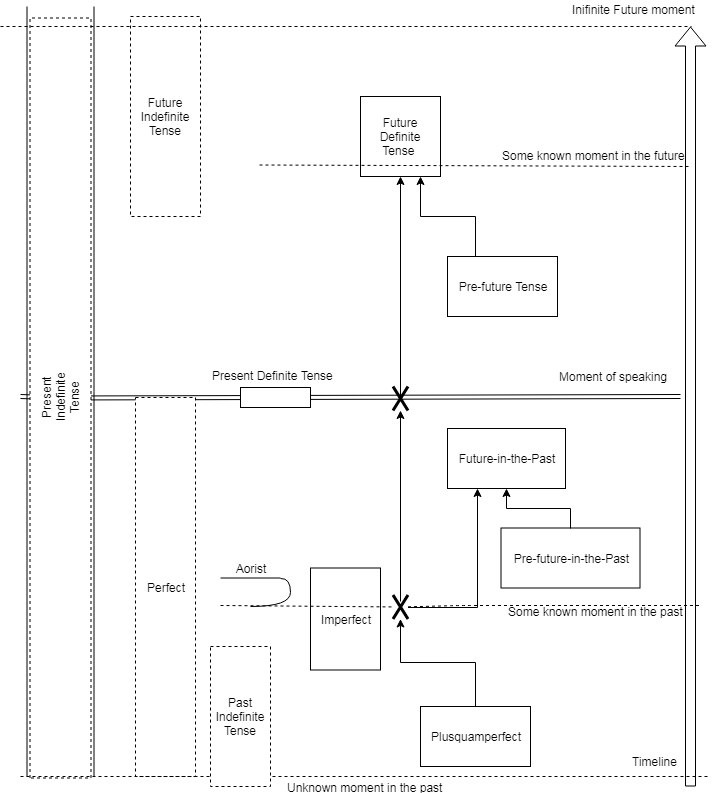
\includegraphics[width=\linewidth]{./sources/tenses.jpg}
	\caption{Tenses in Novoslovnica}
	\label{fig:tenses}
\end{figure}

Present group of tenses consists of Present Indefinite Tense (\textit{Pritomen čas}) and Present Definite Tense (\textit{Sëdyšen čas}).

Present Indefinite Tense\index{tense!present indefinite} (\textit{Pritomen čas}) is used when the action does not depend on time. For example, in the first example we know that the Earth always revolves and nothing but the apocalypsis can change it. This tense is very similar to the English one and has similar use cases. We can find this tense in indicative (examples 1, 2) and declarative (example 3, 4) moods mostly (in some cases it can be found in different moods too).

Note that in declarative there are two variants of present indefinite, because of its resultive semantics. In example 3 you can see the verb in declarative mood, in present indefinite tense, and in example 4 you can see the same tense and mood but within a predicateless sentence.

Also take care of the translation in example 3. You can mess it with English Present Perfect Tense (He has bought two cars), but this sentence should be translated with the verb «to have» in Present Indefinite with the participle III of the verb «to buy» (bought).

\textbf{Examples:}

\textit{Zemlä sę vreta okolo slånca.} - The Earth revolves around the Sun.

\textit{Vsękyǐ denj ja hođam do učilišta prez lěpyǐ park.} — Every day I walk to school through the beautiful park.

\textit{On imá kupeno dva vozidla.} — He has two cars bought.

\textit{Lěs i tïhota...} — There are forest and silence around me...

Present Definite Tense\index{tense!present definite} (\textit{Sëdyšen čas}) is used if the action depends on time. In the first example we can see a sentense with the following semantics: now I think about the rest, though in an hour I can forget about this thought.

Generally, this tense is close to Present Continuous Tense in English, though has a different interpretation. If you want to get in differences, we can give you such an example: «The Earth is revolving around the Sun at the moment». Read this hypothetic sentence that is syntaxicly valid in English.

What would be the differences of English and Novoslovnica here? It is in a term of differentiation. English operates with the time and Novoslovnica operates with the mutability. That is why here Novoslovnica will still use Present Indefinite Tense with the word «sëdy» (at the moment).

\textbf{Examples:}

\textit{Ja myslü o počïvkě.} — I am thinking about the rest.

\textit{On idaje do råboty, zato ne može da odgovori vam.} — He is going to the work, that is why he cannot answer you.

The group of future tenses comprises two ones: Future Tense and Pre-future Tense.

Future Definite Tense\index{tense!future definite} (\textit{Bųdešt čas}) defines that the action will appear in the future with reference with the moment of speaking. There are three variants of how you can use Future Tense in Novoslovnica.

Firstly, you can use the verb «hteti» (to will) in 3-person form with the main verb in Present Indefinite Tense (example 1). This varitant is most similar to English Future Simple Tense.

Secondly, you can use the verb «byti» (to be) with inifinitive form of the main verb (example 2). This variant is close to English Future Continuous Tense. It is often used with verbs of A-type (read the chapter about verbal types in Novoslovnica).

Finally, you can use a synthetic verb form with the future tense conjugation (example 3). In English, it should be translated in Future Simple so as the first one.

\textbf{Examples:}

\textit{Ja hte kazam ti něčto.} — I will tell you something.

\textit{Ja bųdu sluhati gudbu.} — I will listen to music. (I will be listening to music).

\textit{Nakonec ja tę viđahtem}. – Finally, I will meet you.

Pre-future Tense\index{tense!pre-future} (\textit{Predbųdešt čas}) is a grammatical tense that is used when the speaker should explicitly show that the action will take place before another future action. So, this tense deals with the comparison of future actions rather than with the moment of speaking.

In Novoslovnica Pre-future Tense is formed by using the verb «hteti» in 3-person form with the main verb in perfect form (examples 1, 2). This tense should be translated in English with Future Perfect Tense.

\textbf{Examples:}

\textit{Ja hte sòm kupil květy, dy ty hte priǐdaš do města.} — I will have bought flowers, when you come to the place.

\textit{On hte je zakončil učilišto, dy otec mu hte sę vreta dodomu}. — He will have graduated from school, when his father comes back home.

Future Indefinite Tense\index{tense!future indefinite} (\textit{Něĝdašen čas}) is a rather rare tense to be used in Novoslovnica. It has no direct equivalents in English and should be translated in Future Simple with some keywords (such as «somewhen», «ever», «once»). The sense of this tense is to show that the action takes place in a future moment or period of time, but we do not care of when it will occur or how long it will last.
This tense is formed by Pre-future form of the verb «byti» with the past passive participle of the main verb. Look at the examples to get acquainted.

\textbf{Examples:}

\textit{On hte je byl nagrådil medalom mę.} — Once he will grant me with a medal.

\textit{Ja hte sòm byl kupil vašu věčj.} — Once I will but your item.

All other tenses are related to the past period of time. Firstly, we will consider real past tenses and then future-in-the-past ones.

Aorist\index{tense!aorist} (\textit{Prost minul čas}) determines the fact of the committed action without semantic details. It is similar in usage with English Past Simple Tense. Using Aorist we consider only the time the action occurs, but do not think about its duration.

In Novoslovnica it is formed by verb-base vowels with past definite endings: «-h», «-ša», «-še», «-hma», «-hta», «-ha», «-hme», «-hte», «-hu».

\textbf{Examples:}

\textit{Ja dělah råbotu-ta včera.} — I did the work yesterday.

\textit{Pred dvě ročiny ja jěŝih v gråd-òt.} — Two years ago I travelled to the city.

Imperfect\index{tense!imperfect} (\textit{Neporęden minul čas}) determines the imperfect aspect of the past action. That means it is used with habitual, durable repeated actions etc, that took place in the past. Using imperfect we add the information, that our action took some exact time in the past. This tense is similar in usage with English Past Continuous Tense or Past Perfect.

It is formed so as Aorist with the one difference. There is a «-ě-» vowel before endings, not the verb-base vowel. So, for any verb type (see a chapter about verbal types) there is only a single imperfect form.

\textbf{Examples:}

\textit{Ja pišěh nadomnu råbotu dvě godiny včera.} — I was writing my homework for two hours yesterday.

\textit{Prijatelj mi ráděše na zavodu dvě ročiny.} — My friend had worked on a plant for two years.

Perfect\index{tense!prefect} (\textit{Svòršen minul čas}) determines the action has been committed before the present moment. That means, that we take account on the result of the action, on the fact it is finished, while Aorist determines the fact of the action itself and the time when it occured. So, it is a full equivalent of English Present Perfect Tense.

In Novoslovnica Perfect is formed by the auxiliary verb «byti» in Present Indefinite and an L-participle following it.

\textbf{Examples:}

\textit{On je izmyslïl novu ŧeoriju o problemě-ta.} — He has devised a new theory on the problem.

\textit{Môǐ brat je zakončil vysšojučilišto.} — My brother has graduated from University.

Plusquamperfect\index{tense!plusquamperfect} (\textit{Predminul čas}) determines the fact our action is further from us than another action in the past. It is akin Pre-Future tense, just with past actions. Simply speaking, it is an equivalent of English Past Perfect Tense. So as Pre-Future tense, actions in Plusquamperfect are usually used in pair with another past action that stands in Aorist.

Plusquamperfect in Novoslovnica is formed with aorist form of the auxiliary verb «byti» with an L-participle of the main verb.

\textbf{Examples:}

\textit{Ja byh doǐdal do ulicy-ta, dy on mi odŝvoniše, če ne može da priǐde.} — I had arrived to the street by the time he called be to say he cannot come.

\textit{On byše zdělal model, ĝda ja kazaše mu, če to ne máše potrěbnostï.} — He had done a model, when I told him it was unnecessary. 

Now we should consider two last tenses: Future-in-the-Past tense and Pre-Future-in-the-Past tense.

Future-in-the-Past tense (Bųdešt v minulom čas) is used when we speak about past actions, that occured after some other past actions. To emphasize this fact we use a past variant of the future tense — Future-in-the-Past. English has an equivalent, so it is easy to build a parallel between these two tenses. In Novoslovnica this tense is build with imperfect of the auxiliary verb «hteti» and DA-construction of the main verb (example 1).

This tense has also another meaning, that can be expressed with «would like to» phrase in English. It shows a polite intention to do something (example 2).

\textbf{Examples:}

\textit{My zapytahme dali vozidlo htěše da priǐde včas.} — We wondered if the bus would arrive on time.

\textit{Ja htěh da kazam ti něčto.} — I would like to say you something.

Pre-Future-in-the-Past Tense\index{tense!pre-future-in-the-past} (\textit{Predbųdešt v minulom čas}) is used, when we speak about some actions, that happened earlier than some future actions in the past (analogue of pre-future tense in the past). It has a similar meaning with Future-in-the-Past Perfect tense in English and it is rather rarely used.

It is formed with imperfect of the auxiliary verb «hteti» with perfect form of the main verb via DA-construction (look at the example).

\textbf{Examples:}

\textit{Vy kazahte, če htěhte da jeste podpisali pismo pred tym, kak htěhte da započïnate råbotati.} — You said you would have signed the paper before you would start working.

Past Indefinite Tense\index{tense!past indefinite} (\textit{Davnominul čas}) is the last official tense in Novoslovnica. It describes an action that occured in some moment in the past we do not know. In English we should translate it with Past Simple or with the «used to»-construction. It can be considered as a pair to Future Indefinite Tense.

\textbf{Examples:}

\textit{On je byl pisal knigu.} — He used to write a book.

Let us summarize all the equivalents of Novoslovnica's Tenses in English in the next table.

\begin{table}
	\caption{English equivalents of tenses in Novoslovnica}
	\begin{tabular}{ p{11em} p{11em} }
		\textbf{Tense in Novoslovnica}       & \textbf{English equivalent}                  \\
		Present Indefinite Tense             & Present Simple                               \\
		Present Definite Tense               & Present Continuous                           \\
		Future Indefinite Tense              & “once” + Future Simple                       \\
		Future Definite Tense (with “hteti”) & Future Simple                                \\
		Future Definite Tense (with “byti”)  & Future Continuous                            \\
		Future Definite Tense (single form)  & Future Simple                                \\
		Pre-future Tense                     & Future Perfect (Cont.)                       \\
		Future-in-the-Past Tense             & Future-in-the-Past Simple or “would like to” \\
		Pre-future-in-the-Past Tense         & Future-in-the-Past Perfect (Cont.)           \\
		Aorist                               & Past Simple                                  \\
		Perfect                              & Present Perfect (Cont.)                      \\
		Imperfect                            & Past Continuous                              \\
		Plusquamperfect                      & Past Perfect (Cont.)                         \\
		Past Indefinite Tense                & “used to”                                    
	\end{tabular}
\end{table}

The third verbal category can be found in Novoslovnica which is shown only in differences between Aorist and Imperfect: perfection, while other tenses differ only by determinacy and time. So, you can use complex tenses as Perfect, Plusquamperfect, Past Indefinite etc. with aorist and imperfect participles and receive two shades of perfection meaning.

\section{Mood}

% TODO: Check the correspondence with the article

Mood is a grammatical feature of verbs, used for signaling modality []. Mood is distinct from grammatical tense or grammatical aspect, although the same word patterns are used for expressing more than one of these meanings at the same time. There are several moods in Novoslovnica \cite{nsl-naklony}:

\begin{itemize}
	\item Indicative
	\item Declarative
	\item Subjunctive
	\item Conjunctive I
	\item Conjunctive II
	\item Imperative
	\item Optative
	\item Jussive
	\item Hortative
	\item Supine
	\item Inferential
\end{itemize}

Moods are divided into realis and irrealis moods. Realis mood is a grammatical mood which is used principally to indicate that something is a statement of fact. More precisely, it is used to express what the speaker considers to be a known state of affairs. Novoslovnica has two realis moods - indicative and declarative.

Indicative mood (\textit{Oznamitelnyǐ})  is used when we need simply to indicate that something is a statement of fact. Indicative has a variety of forms, including positive, negative and interrogative. Due to this fact it is chosen to be a basic mood, that is compared to the others. Indicative mood will be extensively considered in the next chapters. Just look at few examples.

\textbf{Examples:}

\textit{On glěděše iz prozorca doma si.} - He was looking out of the window of his house.

\textit{Ja bųdu hoditi vò vysšojučilišto črez dvě godiny.} - I will attend the university in two years.

Declarative mood (\textit{Objavitelnyǐ}) is used when we describe a state of something, considering the action it was caused by. Declarative mood is of the same degree of variety as indicative mood, though is not used as often as indicative.

The first difference with indicative mood is in using auxiliary verb “imáti” (to have) instead of “byti” (to be) while forming sentences. This makes some semantic shifts in Novoslovnica. Look at the second example: the auxiliary verb is used in present tense, though it has a resultive semantic value. For present semantics the verbless sentences are used (first example).

The second difference is in the particle being used with the auxiliary verb in two moods. In indicative we use L-particles, while in declarative mood we use passive ones.

\textbf{Examples:}

\textit{Rěka krasna i slånco.} - (There are) Beautiful river and the sun (around me).

\textit{Ja mám rođeno dvôh synoŭ.} - I have two sons born.

Subjunctive mood (\textit{Predpokladnyǐ}) is used when we want to express various states of unreality: wish, emotion, possibility, obligation etc. Subjunctives occur most often, although not exclusively, in subordinate clauses, using particles “aby”, “žeby”, “čtoby”, “išby” (example 1).

Take a note about absence of auxiliary verb while using L-particles. We just use a subjunctive particle with them. Though, we can also use infinitive instead of L-particle with the object in dative (example 2). Moreover, DA-forms can be used to express subjunctive (example 3). Nevertheless, there are cases you can use subjunctive in the main clause (example 4). 

\textbf{Examples:}

\textit{Az upëram aby ty odidal.} - I would like you to leave.

\textit{Az upëram aby ti odidati.} - It’s better for you to leave.

\textit{Ja htem da ty odidaš.} - I want you to leave.

\textit{Ty by odidal odde.} - You better leave here.

Conjunctive mood I (\textit{Domyselnyǐ}) is used to express real wishes relatively present moment. It means, using conjunctive I we show that our wish is still able to be implemented. It is a classic variant of conjunctive and is formed by conjunctive form of the verb “byti” (to be) with an L-participle.

In fact, this mood is rather similar to Conditional II in English with the same tense analogues used (examples 2, 3). If we use just conjunctive clause, it is similar with “wish-construction” usage area in English (example 1). However, we can express conjunctive with the single clause using past transgressive (example 4).

Note, that having two clauses we need to use conditional conjunctions (“ako”, “jestjli”, “koli”, “dali”, “či” etc.).

\textbf{Examples:}

\textit{Az bih htěl da viđu slånco v ovyǐ obvlåčnyǐ denj.} - I wish I see the sun in this cloudy day.

\textit{On biše doǐdal do nas, ako my zazovahme ĝo.} - He would come if we called him.

\textit{Ako znaše on novoslovnicu, mogal biše da govori so vsïmi slověnami.} - If he knew Novoslovnica, he would speak with all Slavs.

\textit{Znavšy novoslovnicu, on mogal biše da govori so vsïmi slověnami}. - If he knew Novoslovnica, he would speak with all Slavs.

Conjunctive mood II (\textit{Domyselnyǐ}) is the second conjunctive mood and it is used to express unreal wishes that have not been realized relatively a moment in the past. It can be formed by the verb “byti” in conjunctive form either  with supine (example 1) or with plusquamperfekt form of the main verb (example 2). It can be related to Conditional III in English. 

Note, that using supine you do not have to use conditional conjunctions between clauses. Moreover, we can use past active participle in the conditional clause (example 3). Attention! Compare this with the past transgressive in the single clause in Conjunctive I.

\textbf{Examples:}

\textit{Htětj da sę vidim s nim včera, bih byl mogal to da sdělam.} - If  I had wanted to see him yesterday, I would have meet him.

\textit{Ako byh htel da sę vidim s nim včera, bih byl mogal to da sdělam.} - If  I had wanted to see him yesterday, I would have meet him.

\textit{Ako byh htel da sę vidim s nim včera, bih byl mogavšym to sdělati.} - the same translation

Imperative mood (\textit{Zapovědnyǐ})  is used when we want to tell somebody a command or a request. In Novoslovnica it has only I-person (in dual and plural) and II-person (in singular, dual and plural) forms. It is indicated by special endings (look forward for details). In the examples you can see how imperative is used.

Please note that imperative is indicated only by single form. Complex forms are not of this mood.

\textbf{Examples:}

\textit{Piši ovu knigu.} - [Please] write this book. (you, sg)

\textit{Kažite mu poslanije-to.} - [Please] tell him the message. (you, pl)

\textit{Pročitaǐte ovu knigu.} - [Please] read this book. (you, pl)

\textit{Predgotuǐmo juž sëdy pokôǐ-ot.} - [Please] prepare the room now! (we, pl)

Optative mood (\textit{Žadatelnyǐ}) is a grammatical mood that expresses wish or hope. It is used when we want something or somebody to let us succeed in any action we are going to do. It is formed by DA-construction in the main clause (look at the examples). 

In English we can find similarity in LET-forms (examples 1, 2) or some general expressions that reveal our wish (example 3).

\textbf{Examples:}

\textit{Da daǐ mi pomognuti ti.} - Let me help you.

\textit{Da bųde tako.} - Let it be so.

\textit{Da žive Bòlĝarija.} - Long live Bulgaria.

Jussive mood (\textit{Umožnitelnyǐ}) is a grammatical mood of verbs for issuing orders and commanding. In Novoslovnica it is used to make orders for third-person expressions. There are no direct equivalents in English for this mood, but we can translate it with impersonal sentences (example 1) or with MUST-modal expressions. It is formed by indicative with “haǐ” modal word.

\textbf{Examples:}

\textit{Haǐ toǐ ne tòpta trevy.} - Do not walk on grass.

\textit{Haǐ on podide.} - He must come closer.

Hortative mood (\textit{Predložnyǐ})  is a grammatical mood that let verb express encourage or discourage of doing something. It can be translated with “let us” (encourage) or “might not” (discourage) constructions in English. In Novoslovnica it is formed with “něhaǐ” modal word with indicative and is able to have negative (example 4) and positive (examples 1-3) form. It is generally used just with I-person expressions.

\textbf{Examples:}

\textit{Něhaǐ grame v ovu gru.} - Let us play this game.

\textit{Něhaǐ pějama pěsnü.} - Let us (both) sing a song.

\textit{Něhaǐ govorim to otcu.} - I might say this to father.

\textit{Něhaǐ ne idame v dom-òt.} - We might not go into the house.


Supine (\textit{Dostęgatelnyǐ}) is rather a grammar form than a mood. Nevertheless, it is often used to express aiming something and the action of approaching to the goal that has been defined. It is similar to infinitive but the ending (infinitive has “-ti” ending, while supine has “-tj” endind). It is usually used with modal verbs and verbs of moving.

Supine can be translated in English through complex predicate. That is because in Novoslovnica supine is practically never used as a single verb form. It is generally used with main verb that determine the background action of the circumstance. Look at the examples to get acquainted with it.

\textbf{Examples:}

\textit{Moǐca je priǐdala povědatj dobru novinu.} - Mojca has come to message a good news.

\textit{Běgi skoro sę preoblekatj.} - Run fast to change clothes.

\textit{Poǐdame kupovatj.} - Let’s go to buy something.

Inferential mood (\textit{Prekazatelnyǐ}) is used to report an unwitnessed event without confirming it. It is often used in stories or fiction books and is very similar with indicative. The only difference is in 3-person in past tenses, where the auxiliary verb “byti” disappears and we use just L-participle. In English it should be translated with ordinary indicative (examples 1-4), sometimes “there”-forms also can be used (example 5). Not, that we use L-participle in Novoslovnica in the past tense (you can mess it with Perfect tense), while it should be translated in Past Simple.
Look at the examples.

\textbf{Examples:}

\textit{Jesòm mu ĝo kupil.} - I have bought it for him.

\textit{Byl sòm kupil naǐ-prosty martenicy, ale toǐ izbral naǐ-råzkošny.} - I had bought simpliest martenitsy, but he bought the most luxurious.

\textit{On byl bogatym.} - He was rich.

\textit{Kųde byl master?} - Where was the master?

\textit{Žila žena i mųž v malomu domu.} - There lived a woman and a man in a small house.

\section{Noun}

\begin{table}[h]
	\caption{Noun characteristics}
	\begin{tabular}{lllll}
		\textbf{Title}              & \textbf{Value}                            \\
		Semantic value              & Concept                                   \\
		Category                    & Independent                               \\
		Subcategory                 & Nominal                                   \\
		Alteration                  & Declension                                \\
		Alteration parameters       & Case, Numbers, Gender, Type of Declension \\
		Differentiation parameters  & Gender, Animacy, Types of  Declension                                  
	\end{tabular}
\end{table}

Nouns can be differentiated by three parameters: gender, animacy and the type of declension.

\underline{Animacy} determines whether the object is animate (we are able to ask “Who is it?” to the object) and inanimate (we are able to ask “What is it?” to the object).

\underline{Gender} determines whether the object is masculine, feminine or undefined (we cannot say it is one of the previous genders). Hence, there are three genders: masculine (with masculine properties), feminine (with feminine properties) and neutral (with undefined properties).

Despite English, Novoslovnica make us always show word gender explicitly of both animacies. We can say “it” to the object if we aren’t coupled with it in English. In Novoslovnica (as in every Slavic language) we should use the predefined gender when we speak about some concept (noun). Using wrong genders shows your ignorance and language nescience.

\underline{Type of declension} is a parameter of declension function. Declension is a function of word alteration. It has two input parameters - the word itself and the type of declension that includes the terms of animacy, gender and some morphological features (such as word endings) in it. The output is a list of forms that the noun can be changed into. Novoslovnica supports 27-cell output list with (3 numbers) * (9 cases) elements in it. Further you can see tables of different declension types. These tables cover all use cases of declension function.

P.S. In tables abbrevs “A” and “I” are for “animate” and “inanimate” respectively.


\begin{table}
	\caption{Hard feminine}
	\begin{tabular}{lllllll}
		\textbf{Ia Type}       
			& \multicolumn{2}{c}{Singular} 
				& \multicolumn{2}{c}{Dual} 
					& \multicolumn{2}{c}{Plural} \\
		& An.   & Inan.  & An.   & Inan.   & An.  & Inan. \\
		Nominative    & \multicolumn{2}{c}{-a}      
						& \multicolumn{2}{c}{-ě}        
							& \multicolumn{2}{c}{-y} \\
		Genitive      & \multicolumn{2}{c}{-y}       
						& \multicolumn{2}{c}{-oŭ}      
							& \multicolumn{2}{c}{-}   \\
		Partitive     & \multicolumn{2}{c}{-y}       
						& \multicolumn{2}{c}{-oŭ}      
							& \multicolumn{2}{c}{-} \\
		Accusative    & \multicolumn{2}{c}{-u}       
						& -ova & -ě
							& \multicolumn{2}{c}{-} \\
		Dative        & \multicolumn{2}{c}{-ě}       
						& \multicolumn{2}{c}{-oma}     
							& \multicolumn{2}{c}{-am} \\
		Instrumental  & \multicolumn{2}{c}{-oǐ}     
						 & \multicolumn{2}{c}{-ama}     
						 	& \multicolumn{2}{c}{-ami} \\
		Prepositional & \multicolumn{2}{c}{-ě}       
						& \multicolumn{2}{c}{-ověh}     
							& \multicolumn{2}{c}{-ěh} \\
		Locative      & \multicolumn{2}{c}{-jï}      
						& \multicolumn{2}{c}{-oŭ}       
							& \multicolumn{2}{c}{-ah} \\ 
		Vocative      & \multicolumn{2}{c}{-o}       
						& \multicolumn{2}{c}{-ove}      
							& \multicolumn{2}{c}{-ije}
	\end{tabular}
\end{table}


\begin{table}
	\caption{Hard masculine}
	\begin{tabular}{lllllll}
		\textbf{Ib Type}       
		& \multicolumn{2}{c}{Singular} 
		& \multicolumn{2}{c}{Dual} 
		& \multicolumn{2}{c}{Plural} \\
		& An.   & Inan.  & An.   & Inan.   & An.  & Inan. \\
		Nominative    & \multicolumn{2}{c}{-a}      
		& \multicolumn{2}{c}{-ě}        
		& \multicolumn{2}{c}{-y} \\
		Genitive      & \multicolumn{2}{c}{-y}       
		& \multicolumn{2}{c}{-oŭ}      
		& \multicolumn{2}{c}{-}   \\
		Partitive     & \multicolumn{2}{c}{-y}       
		& \multicolumn{2}{c}{-oŭ}      
		& \multicolumn{2}{c}{-} \\
		Accusative    & \multicolumn{2}{c}{-u}       
		& \multicolumn{2}{c}{-ě}
		& \multicolumn{2}{c}{-y} \\
		Dative        & \multicolumn{2}{c}{-ě}       
		& \multicolumn{2}{c}{-oma}     
		& \multicolumn{2}{c}{-am} \\
		Instrumental  & \multicolumn{2}{c}{-oǐ}     
		& \multicolumn{2}{c}{-ama}     
		& \multicolumn{2}{c}{-ami} \\
		Prepositional & \multicolumn{2}{c}{-ě}       
		& \multicolumn{2}{c}{-ověh}     
		& \multicolumn{2}{c}{-ěh} \\
		Locative      & \multicolumn{2}{c}{-jï}      
		& \multicolumn{2}{c}{-oŭ}       
		& \multicolumn{2}{c}{-ah} \\ 
		Vocative      & \multicolumn{2}{c}{-o}       
		& \multicolumn{2}{c}{-ove}      
		& \multicolumn{2}{c}{-ije}
	\end{tabular}
\end{table}

\begin{table}
	\caption{Soft feminine}
	\begin{tabular}{lllllll}
		\textbf{Ic Type}       
		& \multicolumn{2}{c}{Singular} 
		& \multicolumn{2}{c}{Dual} 
		& \multicolumn{2}{c}{Plural} \\
		& An.   & Inan.  & An.   & Inan.   & An.  & Inan. \\
		Nominative    & \multicolumn{2}{c}{-ä}      
		& \multicolumn{2}{c}{-ě}        
		& \multicolumn{2}{c}{-ï} \\
		Genitive      & \multicolumn{2}{c}{-ï}       
		& \multicolumn{2}{c}{-öŭ}      
		& \multicolumn{2}{c}{-ëǐ}   \\
		Partitive     & \multicolumn{2}{c}{-ï}       
		& \multicolumn{2}{c}{-öŭ}      
		& \multicolumn{2}{c}{-ëǐ} \\
		Accusative    & \multicolumn{2}{c}{-ü}       
		& \multicolumn{2}{c}{-ě}
		& \multicolumn{2}{c}{-i} \\
		Dative        & \multicolumn{2}{c}{-ě}       
		& \multicolumn{2}{c}{-ëma}     
		& \multicolumn{2}{c}{-äm} \\
		Instrumental  & \multicolumn{2}{c}{-ëǐ}     
		& \multicolumn{2}{c}{-äma}     
		& \multicolumn{2}{c}{-ämi} \\
		Prepositional & \multicolumn{2}{c}{-ě}       
		& \multicolumn{2}{c}{-ëvěh}     
		& \multicolumn{2}{c}{-ěh} \\
		Locative      & \multicolumn{2}{c}{-jï}      
		& \multicolumn{2}{c}{-öŭ}       
		& \multicolumn{2}{c}{-äh} \\ 
		Vocative      & \multicolumn{2}{c}{-ö}       
		& \multicolumn{2}{c}{-ëve}      
		& \multicolumn{2}{c}{-e}
	\end{tabular}
\end{table}

\begin{table}
	\caption{Soft masculine}
	\begin{tabular}{lllllll}
		\textbf{Id Type}       
		& \multicolumn{2}{c}{Singular} 
		& \multicolumn{2}{c}{Dual} 
		& \multicolumn{2}{c}{Plural} \\
		& An.   & Inan.  & An.   & Inan.   & An.  & Inan. \\
		Nominative    & \multicolumn{2}{c}{-ä}      
		& \multicolumn{2}{c}{-ě}        
		& \multicolumn{2}{c}{-ï} \\
		Genitive      & \multicolumn{2}{c}{-ï}       
		& \multicolumn{2}{c}{-öŭ}      
		& \multicolumn{2}{c}{-ëj}   \\
		Partitive     & \multicolumn{2}{c}{-ï}       
		& \multicolumn{2}{c}{-öŭ}      
		& \multicolumn{2}{c}{-ëǐ} \\
		Accusative    & \multicolumn{2}{c}{-ü}       
		& \multicolumn{2}{c}{-ëva}
		& \multicolumn{2}{c}{-ëvi} \\
		Dative        & \multicolumn{2}{c}{-ě}       
		& \multicolumn{2}{c}{-ëma}     
		& \multicolumn{2}{c}{-äm} \\
		Instrumental  & \multicolumn{2}{c}{-ëǐ}     
		& \multicolumn{2}{c}{-äma}     
		& \multicolumn{2}{c}{-ämi} \\
		Prepositional & \multicolumn{2}{c}{-ě}       
		& \multicolumn{2}{c}{-ëvěh}     
		& \multicolumn{2}{c}{-ěh} \\
		Locative      & \multicolumn{2}{c}{-jï}      
		& \multicolumn{2}{c}{-öŭ}       
		& \multicolumn{2}{c}{-äh} \\ 
		Vocative      & \multicolumn{2}{c}{-ö}       
		& \multicolumn{2}{c}{-ëvi}      
		& \multicolumn{2}{c}{-ïe}
	\end{tabular}
\end{table}

\begin{table}
	\caption{Hard masculine}
	\begin{tabular}{lllllll}
		\textbf{IIa Type}       
		& \multicolumn{2}{c}{Singular} 
		& \multicolumn{2}{c}{Dual} 
		& \multicolumn{2}{c}{Plural} \\
		& An.   & Inan.  & An.   & Inan.   & An.  & Inan. \\
		Nominative    & \multicolumn{2}{c}{-}      
		& \multicolumn{2}{c}{-a}        
		& \multicolumn{2}{c}{-y} \\
		Genitive      & \multicolumn{2}{c}{-a}       
		& \multicolumn{2}{c}{-oŭ}      
		& \multicolumn{2}{c}{-ov}   \\
		Partitive     & \multicolumn{2}{c}{-u}       
		& \multicolumn{2}{c}{-oŭ}      
		& \multicolumn{2}{c}{-ov} \\
		Accusative    & -a & -      
		& -ova & -a 
		& -ov & -y \\
		Dative        & \multicolumn{2}{c}{-u}       
		& \multicolumn{2}{c}{-ovi}     
		& \multicolumn{2}{c}{-am} \\
		Instrumental  & \multicolumn{2}{c}{-om}     
		& \multicolumn{2}{c}{-ama}     
		& \multicolumn{2}{c}{-ami} \\
		Prepositional & \multicolumn{2}{c}{-ě}       
		& \multicolumn{2}{c}{-ověh}     
		& \multicolumn{2}{c}{-ěh} \\
		Locative      & \multicolumn{2}{c}{-u}      
		& \multicolumn{2}{c}{-oŭ}       
		& \multicolumn{2}{c}{-ah} \\ 
		Vocative      & \multicolumn{2}{c}{-e}       
		& \multicolumn{2}{c}{-ove}      
		& \multicolumn{2}{c}{-ïe}
	\end{tabular}
\end{table}



\begin{table}
	\caption{Soft masculine}
	\begin{tabular}{lllllll}
		\textbf{IIb Type}       
		& \multicolumn{2}{c}{Singular} 
		& \multicolumn{2}{c}{Dual} 
		& \multicolumn{2}{c}{Plural} \\
		& An.   & Inan.  & An.   & Inan.   & An.  & Inan. \\
		Nominative    & \multicolumn{2}{c}{-j}      
		& \multicolumn{2}{c}{-ä}        
		& \multicolumn{2}{c}{-ï} \\
		Genitive      & \multicolumn{2}{c}{-ä}       
		& \multicolumn{2}{c}{-öŭ}      
		& \multicolumn{2}{c}{-ëǐ}   \\
		Partitive     & \multicolumn{2}{c}{-ü}       
		& \multicolumn{2}{c}{-öŭ}      
		& \multicolumn{2}{c}{-ëǐ} \\
		Accusative    & \multicolumn{2}{c}{-ä}     
		& \multicolumn{2}{c}{-ëva} 
		& \multicolumn{2}{c}{-ëǐ} \\
		Dative		  & \multicolumn{2}{c}{-ü}       
		& \multicolumn{2}{c}{-ëvi}     
		& \multicolumn{2}{c}{-äm} \\
		Instrumental  & \multicolumn{2}{c}{-ëm}     
		& \multicolumn{2}{c}{-äma}     
		& \multicolumn{2}{c}{-ämi} \\
		Prepositional & \multicolumn{2}{c}{-ě}       
		& \multicolumn{2}{c}{-ëvěh}     
		& \multicolumn{2}{c}{-ěh} \\
		Locative      & \multicolumn{2}{c}{-ü}      
		& \multicolumn{2}{c}{-öŭ}       
		& \multicolumn{2}{c}{-äh} \\ 
		Vocative      & \multicolumn{2}{c}{-ü}       
		& \multicolumn{2}{c}{-ëve}      
		& \multicolumn{2}{c}{-ïe}
	\end{tabular}
\end{table}



\begin{table}
	\caption{Hard neutral}
	\begin{tabular}{lllllll}
		\textbf{IIc Type}       
		& \multicolumn{2}{c}{Singular} 
		& \multicolumn{2}{c}{Dual} 
		& \multicolumn{2}{c}{Plural} \\
		& An.   & Inan.  & An.   & Inan.   & An.  & Inan. \\
		Nominative    & \multicolumn{2}{c}{-o}      
		& \multicolumn{2}{c}{-a}        
		& \multicolumn{2}{c}{-y} \\
		Genitive      & \multicolumn{2}{c}{-a}       
		& \multicolumn{2}{c}{-oŭ}      
		& \multicolumn{2}{c}{-}   \\
		Partitive     & \multicolumn{2}{c}{-u}       
		& \multicolumn{2}{c}{-oŭ}      
		& \multicolumn{2}{c}{-} \\
		Accusative    & \multicolumn{2}{c}{-o}     
		& \multicolumn{2}{c}{-a} 
		& \multicolumn{2}{c}{-y} \\
		Dative        & \multicolumn{2}{c}{-u}       
		& \multicolumn{2}{c}{-ovi}     
		& \multicolumn{2}{c}{-am} \\
		Instrumental  & \multicolumn{2}{c}{-om}     
		& \multicolumn{2}{c}{-ama}     
		& \multicolumn{2}{c}{-ami} \\
		Prepositional & \multicolumn{2}{c}{-ě}       
		& \multicolumn{2}{c}{-ověh}     
		& \multicolumn{2}{c}{-ěh} \\
		Locative      & \multicolumn{2}{c}{-u}      
		& \multicolumn{2}{c}{-oŭ}       
		& \multicolumn{2}{c}{-ah} \\ 
		Vocative      & \multicolumn{2}{c}{-e}       
		& \multicolumn{2}{c}{-ove}      
		& \multicolumn{2}{c}{-ïe}
	\end{tabular}
\end{table}

\begin{table}
	\caption{Soft neutral}
	\begin{tabular}{lllllll}
		\textbf{IId Type}       
		& \multicolumn{2}{c}{Singular} 
		& \multicolumn{2}{c}{Dual} 
		& \multicolumn{2}{c}{Plural} \\
		& An.   & Inan.  & An.   & Inan.   & An.  & Inan. \\
		Nominative    & \multicolumn{2}{c}{-ë}      
		& \multicolumn{2}{c}{-ä}        
		& \multicolumn{2}{c}{-ï} \\
		Genitive      & \multicolumn{2}{c}{-ä}       
		& \multicolumn{2}{c}{-öŭ}      
		& \multicolumn{2}{c}{-ëǐ}   \\
		Partitive     & \multicolumn{2}{c}{-ü}       
		& \multicolumn{2}{c}{-öŭ}      
		& \multicolumn{2}{c}{-ëǐ} \\
		Accusative    & \multicolumn{2}{c}{-ë}     
		& \multicolumn{2}{c}{-ä} 
		& \multicolumn{2}{c}{-ï} \\
		Dative		  & \multicolumn{2}{c}{-ü}       
		& \multicolumn{2}{c}{-ëvi}     
		& \multicolumn{2}{c}{-äm} \\
		Instrumental  & \multicolumn{2}{c}{-ëm}     
		& \multicolumn{2}{c}{-äma}     
		& \multicolumn{2}{c}{-ämi} \\
		Prepositional & \multicolumn{2}{c}{-ě}       
		& \multicolumn{2}{c}{-ëvěh}     
		& \multicolumn{2}{c}{-ěh} \\
		Locative      & \multicolumn{2}{c}{-ü}      
		& \multicolumn{2}{c}{-öŭ}       
		& \multicolumn{2}{c}{-äh} \\ 
		Vocative      & \multicolumn{2}{c}{-ü}       
		& \multicolumn{2}{c}{-ëve}      
		& \multicolumn{2}{c}{-ïe}
	\end{tabular}
\end{table}

\begin{table}
	\caption{Soft feminine}
	\begin{tabular}{lllllll}
		\textbf{IIIa Type}       
		& \multicolumn{2}{c}{Singular} 
		& \multicolumn{2}{c}{Dual} 
		& \multicolumn{2}{c}{Plural} \\
		& An.   & Inan.  & An.   & Inan.   & An.  & Inan. \\
		Nominative    & \multicolumn{2}{c}{-j}      
		& -erě & -ě        
		& -eri & -i \\
		Genitive      & -eri & -i 
		& -eröŭ & -öŭ
		& -erëǐ & -ëǐ \\
		Partitive     & -eri & -i 
		& -eröŭ & -öŭ
		& -erëǐ & -ëǐ \\
		Accusative    & -erj & -j     
		& -erëva & -ě
		& -erëǐ & -ï  \\
		Dative		  & -eri & -i
		& -erëma & -ëma 
		& -eräm & -äm \\  
		Instrumental  & -erïü & -ïü     
		& -eräma & -äma   
		& -erämi & -ämi \\
		Prepositional & -erě & -ě   
		& -erëvěh & -ëvěh     
		& -erěh & -ěh \\
		Locative      & -erjï & -j      
		& -eröŭ & -öŭ
		& -eräh & -äh \\
		Vocative      & \multicolumn{2}{c}{-ï}       
		& -erëve & -ëve
		& -erïe & -ïe 
	\end{tabular}
\end{table}

\begin{table}
	\caption{Soft neutral}
	\begin{tabular}{lllllll}
		\textbf{IIIb Type}       
		& \multicolumn{2}{c}{Singular} 
		& \multicolumn{2}{c}{Dual} 
		& \multicolumn{2}{c}{Plural} \\
		& An.   & Inan.  & An.   & Inan.   & An.  & Inan. \\
		Nominative    & \multicolumn{2}{c}{-ę}      
		& -ęta  & -eni        
		& -ęty & -eny \\
		Genitive      & -ęti & -eni 
		& -ętoŭ & -enoŭ
		& -ęt & -en \\
		Partitive     & -ęti & -eni 
		& -ętoŭ & -enoŭ
		& -ęt & -en \\
		Accusative    & -ęto & -ę     
		& -ętova & -ena
		& -ęt & -eny  \\
		Dative		  & -ęti & -eni
		& -ętovi & -enovi 
		& -ętam & -enam \\  
		Instrumental  & -ętëm & -enëm     
		& -ętama & -enama   
		& -ętami & -enami \\
		Prepositional & -ętě & -eně   
		& -ętověh & -enověh     
		& -ętěh & -eněh \\
		Locative      & -ętjï & -enjï      
		& -ętoŭ & -enoŭ
		& -ętah & -enah \\
		Vocative      & \multicolumn{2}{c}{-ų}       
		& -ętove & -enove
		& -ętïe & -ïe 
	\end{tabular}
\end{table}

\section{Adjective}

\begin{table}[h]
	\caption{Adjective characteristics}
	\begin{tabular}{lllll}
		\textbf{Title}              & \textbf{Value}               \\
		Semantic value              & Attribute                    \\
		Category                    & Independent                  \\
		Subcategory                 & Nominal                      \\
		Alteration                  & Declension                   \\
		Alteration parameters       & Case, Number, Gender, Degree \\
		Differentiation parameters  & Gender, Type, Form
	\end{tabular}
\end{table}

Adjective is one of POS that determines an attribute of the concept. There are two types of adjectives - relative and qualitative. 

Relative adjectives are called so, because they show relations between two concepts or a concept and an action.

\textbf{Examples:}

\textit{South (adj) pole} = South (noun) <= relation <= Pole

\textit{Južnyǐ pôl} = Jug <= relation <= Pôl

Qualitative adjectives are called so, because they show the quality of a concept’s property. This quality could be relative or quantitative or purely qualitative (showing concept condition, position, measure etc).

\textbf{Examples:}

\textit{Blue sky} = Sky => is (quality) => blue (attribute)

\textit{Sine nebo} = Nebo => is (quality) => sine (attribute) 

There is the only type of adjective declension. However, we will divide declension tables by gender and base softness.

\begin{table}[!htb]
	\caption{Masculine}
	\begin{tabular}{lllllll}
		\textbf{Masculine}       
		& \multicolumn{2}{c}{Singular} 
		& \multicolumn{2}{c}{Dual} 
		& \multicolumn{2}{c}{Plural} \\
		& Hard   & Soft  & Hard   & Soft   & Hard  & Soft \\
		Nominative    & -yǐ & -ïǐ     
		& -aja  & -äja        
		& -yji & -ïji \\
		Genitive      & -oga & -ëga 
		& -oŭ & -oŭ
		& -yh & -ïh \\
		Partitive     & -ogu & -ëgu 
		& -oŭ & -oŭ
		& -yh & -ïh \\
		Accusative    & -ogo & -ëgo     
		& -aja & -äja
		& -yji* & -ïji*  \\
		Dative		  & -omu & -ëmu
		& -oma & -ëma 
		& -ym & -ïm \\  
		Instrumental  & -ym & -ïm     
		& -yma & -ïma   
		& -ymi & -ïmi \\
		Prepositional & -om & -ëm  
		& -yvěh & -ïvěh     
		& -ěh & -ěh \\
		Locative      & -omu & -ëmu      
		& -oŭ & -oŭ
		& -yh & -ïh \\
		Vocative       & -yǐ & -ïǐ     
		& -aja  & -äja        
		& -yji & -ïji 
	\end{tabular}
\end{table}


\begin{table}[!htb]
	\caption{Feminine}
	\begin{tabular}{lllllll}
		\textbf{Feminine}       
		& \multicolumn{2}{c}{Singular} 
		& \multicolumn{2}{c}{Dual} 
		& \multicolumn{2}{c}{Plural} \\
		& Hard   & Soft  & Hard   & Soft   & Hard  & Soft \\
		Nominative    & -aja & -äja     
		& \multicolumn{2}{c}{-ěja}        
		& -yje & -ïje \\
		Genitive      & -oji & -ëji
		& -oŭ & -öŭ
		& -yh & -ïh \\
		Partitive    & -oji & -ëji
		& -oŭ & -öŭ
		& -yh & -ïh \\
		Accusative    & -uju & -üju     
		& \multicolumn{2}{c}{-ěja} 
		& -yje* & -ïje*  \\
		Dative		  & -oǐ & -ëǐ
		& -oma & -ëma 
		& -ym & -ïm \\  
		Instrumental  & -oju & -ëju
		& -yma & -ïma   
		& -ymi & -ïmi \\
		Prepositional  & -oǐ & -ëǐ
		& -yvěh & -ïvěh     
		& -ěh & -ěh \\
		Locative      & -oji & -ëji      
		& -oŭ & -oŭ
		& -yh & -ïh \\
		Vocative      & -aja & -äja     
		& \multicolumn{2}{c}{-ěja}        
		& -yje & -ïje 
	\end{tabular}
\end{table}

\begin{table}[!htb]
	\caption{Neutral}
	\begin{tabular}{lllllll}
		\textbf{Neutral}       
		& \multicolumn{2}{c}{Singular} 
		& \multicolumn{2}{c}{Dual} 
		& \multicolumn{2}{c}{Plural} \\
		& Hard   & Soft  & Hard   & Soft   & Hard  & Soft \\
		Nominative    & -oje & -ëje     
		& -aja  & -äja        
		& -yje & -ïje \\
		Genitive      & -oga & -ëga 
		& -oŭ & -oŭ
		& -yh & -ïh \\
		Partitive     & -ogu & -ëgu 
		& -oŭ & -oŭ
		& -yh & -ïh \\
		Accusative    & -ogo & -ëgo     
		& -aja & -äja
		& -yji* & -ïji*  \\
		Dative		  & -omu & -ëmu
		& -oma & -ëma 
		& -ym & -ïm \\  
		Instrumental  & -ym & -ïm     
		& -yma & -ïma   
		& -ymi & -ïmi \\
		Prepositional & -om & -ëm  
		& -yvěh & -ïvěh     
		& -ěh & -ěh \\
		Locative      & -omu & -ëmu      
		& -oŭ & -oŭ
		& -yh & -ïh \\
		Vocative       & -oje & -ëje     
		& -aja  & -äja        
		& -yje & -ïje 
	\end{tabular}
\end{table}

\subsection{Full and short adjectives}

There are two forms of adjectives: full and short.

We can find differences in using short and full forms of adjectives only in some cases - Nominative and Accusative. In other cases short adjectives correspond with appropriate full form adjective.

To understand how to change a full adjective to receive its short form look at the next table (C is for “consonant”, V is for “vowel”).

\begin{table}
	\begin{tabular}{ll}
		Full form adjective endings & Short form adjective endings \\
		C + C + yǐ & C + ò C \\
	    V + C + yǐ & V + C \\
		aja & a \\
		oje  & o \\
		yje & y \\
	\end{tabular}
\end{table}

Etymologically full adjectives date back to combined form of an adjective itself (short form) and a pronoun \footnote{Such a phenomenon existed in Russia, Belorussian and Baltic languages. A similar phenomenon is used in Macedonia today. Though a "pronoun-article" is used mostly with verb as in the following sentence.}. 

What about using full and short adjectives… There are some recommendations that you should follow in your speech. I tried to unite them into one table with cases when you should use either full form or short one.

\begin{table}
	\begin{tabular}{ll}
		Full form & Short form \\
		Before the modified noun & In a complex predicate \\
		In denominative sentence & - \\
	\end{tabular}
\end{table}


\subsection{Degrees of comparison}

When we speak about qualitative adjectives, we use a term of a degree of comparison. It’s the condition whether temporal adjective is greater in its measure than another one or not. There are three degrees: positive, comparative and superlative.

\underline{Positive} (or neutral, basic) degree is used when we do not mind about the comparison with other attributes. We could call it an undefined degree.

\underline{Comparative} degree is used when our attribute is greater than another one (attributes must be comparable).  

\underline{Superlative} degree is used when our concept has the attribute with most valuable degree in considered area.

There are two ways of comparison - synthetic and analytic. Synthetic comparison changes the word itself, while analytic comparison uses analytic constructions with other words to create a degree of comparison. You can you both analytic or synthetic comparison forms in your speech.

\textbf{Synthetic comparison}

Comparative degree can be formed in two ways: 

\begin{itemize}
	\item Adding between word base and word ending “-š-”, that means that the attribute has a more strongly pronounced property than another concept, expressed by a noun.
	\item Adding suffix “-š-” plus suffix “-ëǐ-” for soft word base and suffix “-aǐ-” for hard word base before it.
\end{itemize}

\textbf{Examples:}

Bolïǐ – boljšyǐ. Mnogyǐ - mnogšyǐ. Vëlïkyǐ - vëlïkšyǐ.

Bolïǐ – bolëǐšyǐ. Mnogyǐ - množaǐšyǐ. Vëlïkyǐ - vëlïčaǐšyǐ.

Superlative degree also has two variants, that are formed by adding a prefix “-naǐ-” to the comparative form. This prefix has a similar meaning with the English word “most”.

\textbf{Examples:}

Bolïǐ – boljšyǐ - naǐboljšyǐ. Mnogyǐ - mnogšyǐ - naǐmnogšyǐ. Vëlïkyǐ - vëlïkšyǐ - naǐvëlïkšyǐ.

Bolïǐ – bolëǐšyǐ - naǐbolëǐšyǐ. Mnogyǐ - množaǐšyǐ - naǐmnožaǐšyǐ. Vëlïkyǐ - vëlïčaǐšyǐ - naǐvëlïčaǐšyǐ.

Some says Novoslovnica has five degrees of comparison instead of three degrees with doubly forms. Let us know this classification.

\begin{itemize}
	\item \textit{Positive} degree equals to the one in ordinary classification. (Bolïǐ)

	\item \textit{Defined Comparative} degree matches the first variant of comparative form in ordinary classification. It is used when there are two objects and the temporal one has a prevailed property to another one. (\textit{Bolïšyǐ})

	\item \textit{Undefined Comparative} degree matches the second variant of comparative form in ordinary classification. It is used when we have some objects (more than two) and temporal object has a prevailed property to a few objects in the set (probably its power is an undefined number). (\textit{Bolëǐšyǐ})

	\item \textit{Relative superlative} degree matches the first variant of superlative form in ordinary classification. It is used when temporal object is in the set and has a superior property in it, but we cannot say that this property would have a superior value in other sets. (\textit{Naǐboljšyǐ})

	\item \textit{Absolute superlative} degree matches the second variant of superlative form in ordinary classification. It is used when there are no doubts in superiority of the temporal object’s property. (\textit{Naǐbolëǐšyǐ})
\end{itemize}

\textbf{Analytic forms}

There are two variants of how to use analytic comparison of adjectives: to use prefixes or to use an auxiliary adverb.

To create a comparative or a superlative form you should add a prefix “po-” or “naǐ-” respectively to the word though a defis.

\textbf{Examples:}

Kråtkyǐ - po-kråtkyǐ - naǐ-kråtkyǐ

Sïlnyǐ - po-sïlnyǐ - naǐ-sïlnyǐ

Analytic comparison forms have only three ones - positive, comparative and superlative. Analytic comparison with an auxiliary adverb is formed by adding to the positive form of the adjective a comparative or a superlative form of an auxiliary adverb (look at the paragraph about adverb degrees of comparison). However, you cannot use analytic comparison with adjectives “bolïǐ” and “mënïǐ”, because they are the basic forms of these auxiliary adverbs.

\textbf{Examples:}

Kråtkyǐ - bolěǐ kråtkyǐ - naǐbolěǐ kråtkyǐ

Bolïǐ - bolěǐ bolïǐ (\textbf{you cannot do that}!)

\section{Pronoun}

\begin{table}[!hbt]
	\caption{Pronoun characteristics}
	\begin{tabular}{lp{12em}}
		\textbf{Title}              & \textbf{Value}               \\
		Semantic value              & Attribute, Concept           \\
		Category                    & Independent                  \\
		Subcategory                 & Nominal                      \\
		Alteration                  & Declension                   \\
		Alteration parameters       & Case, Numbers, Gender, Person\\
		Differentiation parameters  & Gender, Type, Group
	\end{tabular}
\end{table}

Pronoun\index{pronoun} is a POS that has different meanings. It can play the role of an attribute or a concept, depending on what is replaced with the pronoun. However, pronoun has a verbal property of person.

Pronouns are divided into three types: nominal\index{pronoun!nominal} (noun-like declension), substantive\index{pronoun!substantive} (substantive declension), attributive\index{pronoun!attributive} (adjective-like declension).

There are also several groups of pronouns, depending on their semantic value. They are: personal, possessive, interrogative, relative, indefinite, definitive, reflexive, demonstrative, negative, reciprocal.

\subsection{Personal pronouns}

Personal pronouns\index{pronoun!personal} are one of the most important groups in the Pronoun POS. They replace nouns in sentences when we try to avoid an unreasonable repeat. Personal pronouns have different forms for every person-number cell. In the table you can see them.

\begin{table}[!htb]
	\begin{tabular}{llll}
		& Singular & Dual & Plural \\
		1 person & Ja (Az) & Ma & My \\
		2 person & Ty & Va & Vy \\
		3 person, ms & On & Ona & Oni \\
		3 person, fm & Ona & One & Oně \\
		3 person, neu & Ono & Oná & Onji
	\end{tabular}
\end{table}

I should mention the form “Vy” (You). As in English or polite Russian, we can use this pronoun for a single person when we want to emphasize our respect to the interlocutor. Moreover, we also have to use a plural form of the verb while speaking “Vy” in polite form.

Also you can see two forms of the 1 person - singular pronoun (I). Etymologically the form “Az” is full while “Ja” is only a short one. However, different Slavic languages have retained different forms and now we see Novoslovnica should support both ones. In Novoslovnica the difference between using “Az” and “Ja” lies in phonetics. As you see, “Az” begins with the vowel and ends with a consonant, “Ja” - controversially. If we remember rule 1 we will get such a list of rules:

\begin{itemize}
	\item If the word before the pronoun ends with a vowel and the word after begins with a consonant - you should use “Ja”
	\item If the word before the pronoun ends with a consonant and the word after begins with a vowel - you should use “Az”
	\item In other cases you can use either one or another variant\footnote{“Az” is more formal than “Ja”. In everyday speech you should use "Ja" variant while in scientific, official only "Az" should be used.}
\end{itemize}

Now let us speak about declension of personal pronouns. Personal pronouns relate to nominal pronouns (with noun-like declension). This is the most difficult type to learn.\footnote{The declension of personal pronouns is derived mostly from old-Slavonic language except for 1 person dual. The similar declension within still languages can be found in Slovenian.} But everything has its order and beauty.

Look for the tables in the eighth chapter.

\subsection{Reflexive pronoun}

This\index{pronoun!reflexive} is a separate group of pronouns. There is the only reflexive pronoun in Novoslovnica - “sebę”. Its feature is the absence of nominative form. It has only 7 cases to be alternated. Vocative and Nominative are absent.

\begin{table}[!htb]
	\begin{tabular}{lll}
		Case & Full & Short \\
		Genitive & Sebę & Sę \\
		Partitive & Sebä & Sä \\
		Accusative & Sebe & Se \\
		Dative & Sebi & Si \\ 
		Insrumental & Sobom (Soboǐ) & - \\ 
		Prepositional & O sobě & - \\
		Locative & V sobu & -
	\end{tabular}
\end{table}


“\textit{Sę}” is used very often as a reflexive suffix in verbs. It determines a way of creating medial voice sentences (look the paragraph about it).

However, there is a term of a complex reflexive form (CRF) also. It is formed by the sequence of a personal pronoun and the definitive pronoun “sám”. This form shows a partly-developed reflection of a subject.  

\textbf{Examples:}

\textit{On sám stroji búdu-ta.} -

\textit{On sę stroji.}

\textit{Búda-ta sę stroji nim.}

There is practically no difference in using a reflexive pronoun or a complex reflexive form. However, it is recommended to us a CRF for Nominative and to use a reflexive pronoun in other cases.

\subsection{Possessive pronouns}

Possessive\index{pronoun!possessive} pronouns show whom any object belongs to. For example, we can say “\textit{It is a thing of Bob} (which Bob possesses)”. In Novoslovnica you can use a similar expression: “\textit{To je věčj Boba}” (remember rules of case using). Also Novoslovnica has another expression with a possessive adjective: “To je Bobóva věčj”. This adjective shows that this thing belongs to Bob. However, if we have already used the name of Bob in our sentence, we should not repeat it again. English also uses possessive pronouns in such cases: “\textit{Bob is my friend and that’s his thing}”. We do not repeat the word Bob, we just say - his (which he possesses). That is what the possessive pronouns look like.

These pronouns are attributive, so we have no need to rewrite their declension, just to name nominative forms. Further, you take a nominative form of a possessive pronoun, look through declension tables for adjectives and transform your pronoun so as you did it with an adjective. Now let us look at the nominative forms of possessive pronouns.

\begin{table}[!htb]
	\caption{Possessive pronouns}
	\begin{tabular}{llll}
		& Singular & Dual & Plural \\
		1 person & Môǐ & Naš & Naš \\
		2 person & Tvôǐ & Vaš & Vaš \\
		3 person, ms & Jegôǐ & Onyš & Ih \\
		3 person, fm & Jejôǐ & Oneš & Ih \\
		3 person, neu & Jegôǐ & Onyš & Ih
	\end{tabular}
\end{table}

There also exists possessive adjectives you can see on the next table.

\begin{table}[!htb]
	\caption{Possessive adjective}
	\begin{tabular}{llll}
		& Singular & Dual & Plural \\
		1 person & Môǐnyǐ & Našnyǐ & Našnyǐ \\
		2 person & Tvôǐnyǐ & Vašnyǐ & Vašnyǐ \\
		3 person, ms & Jegôǐnyǐ & Onyšnyǐ & Ihnyǐ \\
		3 person, fm & Jejôǐnyǐ & Onešnyǐ & Ěhnyǐ \\
		3 person, neu & Jegôǐnyǐ & Onyšnyǐ & Ihnyǐ
	\end{tabular}
\end{table}

Possessive adjectives are used only in full form to underline the importance of something. Usually, possessive pronouns should be used.

Look at the examples to see the differences.

\textit{Môǐ pes lübi męso} - My dog likes meet.

\textit{Môǐnyǐ pes lübi męso} - My dog (that we are talking about now) likes meet.

Possessive forms (adjectives and pronouns) should be placed right before the identified word. Nevertheless, you can use a postfix form to describe possessiveness. In that case, you should use personal pronoun in Dative in role of a possessive one. Look at the examples.

\textit{Daǐte moju knigu - Daǐte knigu mi} (the latter is not recommended due to possible misunderstanding)

\textit{Ja  sòm poslal syna mi do pěkarnï - Ja sòm poslal mojoga syna do pěkarnï.}

As you see, such a form does not decline along with the main word. In the following table you can find the correlations between declinable prefix form and a "frozen" postfix one.

\begin{table}[!htb]
	\begin{tabular}{ll}
		\textbf{Prefix} & \textbf{Postfix} \\
		Môǐ & Mi \\
		Tvôǐ & Ti \\
		Svôǐ & Si \\
		Jegôǐ & Mu \\
		Jejôǐ & Ji \\
		Naš & Nam / Nama \\
		Vaš & Vam / Vama \\
		Jih & Jim \\
		Onyš & Onama \\
		Oneš & Oněma \\
	\end{tabular}
\end{table}

Note that the postfix form is pretty similar with use of genitive. The dative possessive form is used mostly in fiction texts to underline the beauty of writing. However, dative for singular pronouns is more frequently used than the genitive one.

\textbf{Examples:}

\textit{To je moja kniga} (Possessive pronoun) - Frequently used

\textit{To je kniga mi} (Dative) - Frequently used

\textit{To je kniga mę} (Genitive) - Rarely used

\textit{On je syn naju} (Genitive) - Frequently used

\textit{On je naš syn} (Possessive pronoun) - Frequently used

\textit{On je syn nama} (Dative) - Rarely used

\subsection{Interrogative and relative pronouns}

Interrogative\index{pronoun!interrogative} pronouns are used when we create a question. They are never in plural or dual. Also they have no declension. The only role of interrogative pronouns is to reveal an aim of the question (How much? Who? What?) - to guide the interlocutor to the right answer (you need).

Relative\index{pronoun!relative} pronouns aim is to introduce a relative clause.

\textit{Relative clause}\index{clause!relative} is a special kind of subordinate clause whose primary function is as modifier to a noun or nominal. We examine the case of relative clause modifiers in NPs first, and then extend the description to cover less prototypical relative constructions.\cite{english-grammar}

Interrogative and relative pronouns are practically the same, only usage differs, that is why I talk about them in the same paragraph. Let us look at them in the table.

\begin{table}[!htb]
	\begin{tabular}{p{8em}p{8em}p{8em}}
		English equivalent & Interrogative pronoun & Relative pronoun \\
		Who & Kto? & Ke \\
		What & Čto & Če \\
		What & Kakyǐ? & Kak \\
		Which & Ktoryǐ? & Ktor \\
		Whose & Čyǐ? & Čyǐ \\
		What & Jakyǐ? & Jak \\
		What & Kakvyǐ ? & Kakòv \\
		What & Kolïkyǐ ? & Kolïk 
	\end{tabular}
\end{table}

Pronouns “Kto”, “Čto” have a similar declension with possessive pronouns. Other pronouns decline so as adjectives do.
  
\subsection{Indefinite and negative pronouns}

Another group of pronouns that are similar to each other are indefinite\index{pronoun!indefinite} and negative\index{pronoun!negative} pronouns. They are derived from interrogative pronouns by adding the negative “ni-” and the indefinite “ne-” prefixes. Their declension equals to their ancestor’s one.

\begin{table}[!htb]
	\begin{tabular}{p{8em}p{8em}p{8em}}
		Interrogative pronoun & Negative pronoun & Indefinite pronoun \\
		Kto? & Nikto & Někto \\
		Čto & Ničto & Něčto \\
		Kakyǐ? & Nikakyǐ & Někakyǐ \\
		Ktoryǐ? & Niktoryǐ & Něktoryǐ \\
		Čyǐ? & Ničyǐ & Něčyǐ 
	\end{tabular}
\end{table}

\subsection{Demonstrative pronouns}

Demonstrative\index{pronoun!demonstrative} pronouns are usually used to make the interlocutor pay attention to something.
There are only four demonstrative pronouns. And this topic is closely connected with the articles. In the table 4.20 you can see these pronouns, divided by the terms of visibility and distance of the object with respect of the speaker.


\begin{table}[!htb]
	\caption{Demonstrative pronouns}
	\begin{tabular}{lll}
		& Visible & Invisible \\
		Far & Onyǐ & Tyǐ \\
		Close & Ovyǐ & Sïǐ  
	\end{tabular}
\end{table}

These pronouns decline so as adjectives do, so that is very easy. Nouns that are used with demonstrative pronouns should not be determinized with article. You should use \underline{either} demonstrative pronoun or articles.

\textbf{Examples:}

\textit{Onyǐ stol je starym} - That table (you are looking at) is old.

\textit{Stol-òn je star} - The table is old.

\textit{Ova kniga je korystnoǐ} - This book is interesting.

\textit{Kniga-va je korystna} - The book is interesting.

\subsection{Attributive pronouns}

Attributive\index{pronoun!definitive} pronouns indicate a generalized feature of an object. 

\begin{table}[!htb]
	\caption{Attributive pronouns}
	\begin{tabular}{ll}
		English equivalent & Definitive pronoun \\
		Whole & Vesj \\
		All & Vsë, vsä, vsï \\
		Every & Vsękyǐ, lübyǐ \\
		Each & Káždyǐ \\
		Another, other & Ïnyǐ, drugyǐ \\
		Both & Oba, obě \\
		Reflexive pronouns & Personal pronouns + sám
	\end{tabular}
\end{table}

All these pronouns decline as adjectives. I should say just about the last one - the pronoun “sám”. This pronoun is used with personal pronouns to create a complex reflexive form (look paragraph about reflexive pronouns). However, it keeps adjective-like declension.

\subsection{Reciprocal pronouns}


The last type of pronouns is reciprocal\index{pronoun!reciprocal}. It is used to refer to a noun phrase mentioned earlier in a sentence. English has only two such pronouns - each other and another one.

Slavic languages have much more variants:

\textit{Drug so drugom} - With each other

\textit{Drug drugu} - Each other

\textit{Raz za razom} - Time by time

\textit{Jeden za drug} - One by one

\textit{Vsęk sò vsęk} - Everyone with everyone

\textit{Et cetera...}

The number of pronouns is formed because of different prepositions and combinations of "vsęk", "jeden", "drug", "raz" used.

\section{Adverb}

\begin{table}[h]
	\caption{Adverb characteristics}
	\begin{tabular}{ll}
		\textbf{Title}              & \textbf{Value}      \\
		Semantic value              & Attribute           \\
		Category                    & Independent         \\
		Subcategory                 & Nominal             \\
		Alteration                  & Comparison          \\
		Alteration parameters       & Degree              \\
		Differentiation parameters  & Type, Group
	\end{tabular}
\end{table}

There are different words that cannot be alternated. The biggest class of such words is adverb. It unites a number of groups adverbs can be divided into.

First of all, you should know that adverbs\index{adverb} can be divided into three types, depending on the form they have: \textit{primary} (P), \textit{secondary} (S) and \textit{derivative} (D). When we speak about adverb groups, these letters will be written next to the adverb to help you easier differentiate these types.

\textit{Primary\index{adverb!primary}} adverbs have been formed long ago and we study it as a whole word, without an easy-found root.

\textit{Secondary\index{adverb!secondary}} adverbs have been formed from two words (or a phrase) or from a frozen word form. 

\textit{Derivative\index{adverb!derivative}} adverbs have been shifted semantically from an adjective. It is the most common type of adverbs.

Now let us talk about groups of adverbs. One distinguishes two main types of adverbs: \textit{Significant} and \textit{Demonstrative}. Significant adverbs names concrete property or process attributes, while demonstrative adverbs only refer to these attributes or have an indication of the common nature.

\begin{figure}
	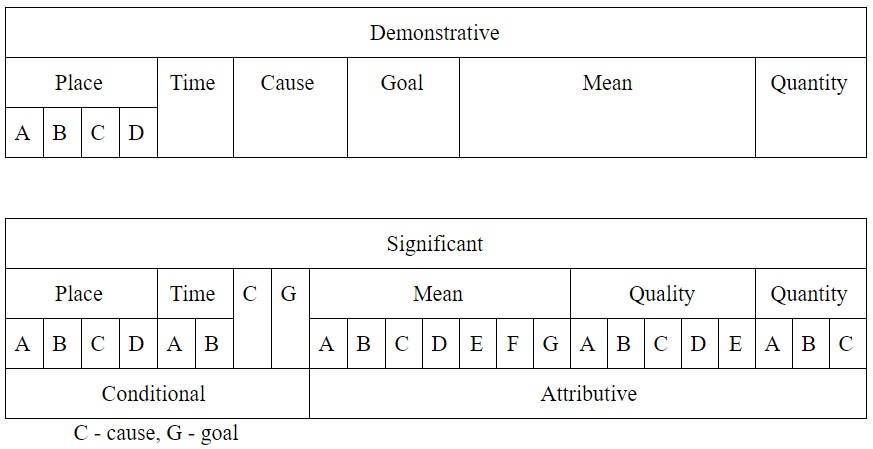
\includegraphics[width=\linewidth]{./sources/adverbs.jpg}
	\caption{Categories of adverbs}
	\label{fig:adverbs}
\end{figure}

\subsection{Demonstrative adverbs}

There are six categories of demonstrative\index{adverb!demonstrative} adverbs. They are adverbs of place, time. cause. goal, mean, quantity.

1. \textbf{Demonstrative adverbs of place.}

Let’s speak about subcategories of this adverbs. 

A. \textit{Adverbs indicating the place of action.}

Question: \textit{Where? (Kųde?)}

Here - \textit{Tut, zdě}

There - \textit{Tamo}

Everywhere - \textit{Vsëde, vsüdu, vsëkųde}

Nowhere - \textit{Nide, nikųde}

Somewhere - \textit{Něde, někųde}

B. \textit{Adverbs indicating the place where action is directed. }

Question: \textit{Whither? (Kųda?)}

Here

There

Everywhere

Nowhere

Somewhere


C. \textit{Adverbs indicating the place of action’s start.}

Question: \textit{Whence? (Odkųde?)}

Here

There

Everywhere

Nowhere

Somewhere


D. \textit{Adverbs indicating the place of action’s start.}

Question: \textit{Where? How far? (Dokųde?)}

(Up to) here

There

Everywhere

Nowhere

Somewhere


2. \textbf{Demonstrative adverbs of time}

Question: \textit{When? (Koĝda?)}

Now

Afterwards

Later

Then

Once

Sometimes

Ever

Never


3. \textbf{Demonstrative adverbs of cause}

Question: \textit{Why? (Čomu?)}

Therefore

Because

Thus

Somehow

Once


4. \textbf{Demonstrative adverbs of goal}

Question: \textit{For what? (Za čto?)}

For

In order to

So as to


5. \textbf{Demonstrative adverbs of mean}

Question: \textit{How? (Kako?)}

So

Likewise

Somehow

Otherwise

Nohow

Like that

That way

Anyhow

Differently


6.\textbf{ Demonstrative adverbs of quantity}

Question: \textit{How much? (Kolïko?)}

So much

Few

Some

Several

Nary


\subsection{Significant adverbs}

Significant\index{adverb!significant} adverbs are often divided into two large subcategories - conditional and attributive adverbs. \textit{Conditional} adverbs shows the conditions of the action took place - place, time, cause, goal. \textit{Attributive} shows the attributes of the action - the mean of the action. its quality and its quantity.

1. \textbf{Significant adverbs of place.}

A. \textit{Adverbs indicating the place of action.}

Question: \textit{Where? (Kųde?)}

Next to (close to)

Ahead

Opposite

Around

Far

Not far

Among

Between

At home

Upstairs

Downstairs


B. \textit{Adverbs indicating the place where action is directed. }

Question:\textit{ Whither? (Kųda?)}

Ahead

To the right

Upwards

Sideways

Downwards

Opposite

Home


C. \textit{Adverbs indicating the place of action’s start.}

Question: \textit{Whence? (Odkųde?)}

From upstairs

From downstairs

From the right

From the left


D. \textit{Adverbs indicating the place of action’s start.}

Question: \textit{Where? How far? (Dokųde?)}

(Up to) here

There

Everywhere

Nowhere

Somewhere


2. \textbf{Significant adverbs of time}

Question: \textit{When? (Koĝda?)}

Now

Afterwards

Later

Then

Once

Sometimes

Ever

Never


3. \textbf{Significant adverbs of cause}

Question: \textit{Why? (Čomu?)}

Therefore

Because

Thus

Somehow

Once


4. \textbf{Significant adverbs of goal}

Question: For what? (Za čto?)

For

In order to

So as to


Further let’s speak about attributive significant pronouns.

1. \textbf{Significant adverbs of mean}

Question: \textit{How? (Kako?)}

So

Likewise

Somehow

Otherwise

Nohow

Like that

That way

Anyhow

Differently

2. \textbf{Significant adverbs of quality}


3.\textbf{ Significant adverbs of quantity}

Question: \textit{How much? (Kolïko?)}

So much

Few

Some

Several

Nary

\subsection{Degrees of comparison}

Likewise adjectives, adverbs have three degrees of comparison\index{comparison}. Moreover, there are synthetic analytic forms too. 

Remember (look at paragraph about adjective degrees of comparison), that there ar three degrees: positive, comparative and superlative.

\textbf{Synthetic forms}

Comparative\index{comparison!synthetic} form is made by adding to the word base the suffix “ěǐ’. Unlike adjectives, this is the only suffix to create a comparative form (compare with suffixes “ëǐ”, “aǐ” for hard and soft bases in adjectives). 

\textbf{Examples:}

\textit{Mnogo - Množěǐ}

\textit{Sïnë - Sïněǐ}

Superlative form is made so as it is in adjectives - adding a suffix “naǐ-” to the comparative form.

\textbf{Analytic forms}

Analytic\index{comparison!analytic} forms provide simple ways of creating comparative and superlative forms without modifying the word itself. There two types of adverb analytic comparison.

\textbf{Using prefixes}

Comparative form is created by adding prefix “po-” through a defis ro a positive form. Superlative form is created by adding prefix “naǐ-” through a defis to the positive form.

\textbf{Examples:}

\textit{Mnogo - po-mnogo - naǐ-mnogo}

\textbf{Using an auxiliary adverb}

To the positive form you should add an auxiliary adverb in comparative or superlative form.

\begin{table}
	\begin{tabular}{lll}
		Auxiliary adverb
		& Comparative form
		& Superlative form \\
		more & bolěǐ & naǐbolěǐ \\
		less & mëněǐ & naǐmëněǐ \\
	\end{tabular}
\end{table}

\textbf{Examples:}

\textit{Mnogo - bolěǐ mnogo - naǐbolěǐ mnogo}

You can use synthetic and analytic forms at the same time.

\section{Predicative}

\begin{table}[!htb]
	\caption{Predicative characteristics}
	\begin{tabular}{ll}
		\textbf{Title}              & \textbf{Value}                            \\
		Semantic value              & Predicate                                 \\
		Category                    & Independent                               \\
		Subcategory                 & Nominal                                   \\
		Alteration                  & None                                      \\
		Alteration parameters       & None                                      \\
		Differentiation parameters  & Tense                                  
	\end{tabular}
\end{table}

Predicative\index{predicative} is a POS that is closely deriving to the predicate. Formally, it is an adverb that plays the role of the predicate (concluded in the predicate as a part of it). 

You should divide a syntax and morphological definitions of predicative. Now we are talking about the second one. In russian philology you can find the term of “condition category” - the equivalent for predicative (morphological definition). In this paragraph we will speak just about this term.

Predicative determines the class of words indicating an attribute or a condition of a person, environment etc., especially mental. Predicatives cannot be alternated, though they can be differentiated by tenses using an auxiliary verb “to be”. 

Predicatives have homonyms with adverbs, and nouns.  

\textbf{Examples:}

\textit{Ona hlådno mi kazala, če ne hoče da vidi mę} - She coldly said to me she does not want to see me (Adverb)

\textit{Dnësj je hlådno.} - It is cold today. (Predicative)

The most popular case of using predicative are modal constructions like "it is necessary", "it is needed" in passive form. Look at the following examples to compare active and passive forms.

\textit{Ja trěbam idati v còrkvu} - I should go to the church

\textit{Je nuđno mi da idam v còrkvu.} -  It is necessary for me to go to the church
\section{Verb}

Verb\index{verb} is a POS that describes the predicate and its properties. 


\subsection{Verbal types}

Learning Slavic languages you could mention that there is a set of verb suffixes that is very eliminated. Novoslovnica provides a theory that allows you to construct a right verb form.
Verbs with different verb suffixes represent different verbal types. There are four types of verbs in Novoslovnica.

\begin{itemize}
	\item A-type\index{verb!a-type}: verbs of this type define that the action in common sense.  
	\item E-type\index{verb!e-type}: verbs of this type define that the action is long-termed.
	\item I-type\index{verb!i-type}: verbs of this type define that the action is short-termed. This type comprises verbs with suffixes I and O. The suffix O is used when the consonant before the constructed suffix is involved in alterations depending on soft vowels that the vowel I is.
	\item U-type\index{verb!u-type}: verbs of this type define that the action is dotty.
	\item Extra type\index{verb!extra-type}. Is formed with the suffix “-OVA-” and defines the repeated action.  
\end{itemize}

When you speak about the action, you find what characteristic is suitable for the action and then use one of the predefined verbal types.

Somebody can ask what are the differences in tenses and types, because it might be confusing. However, verbal type determines the durability of the action (or its repeating property) while tense determines tense characteristic of the action such as completeness, stability in time, result, order etc.

All tenses provide difference between conjugation of different verbal types except imperfect. This tense has the common conjugation table for all verbal types. 

Further we will speak about conjugation itself. We will look at verb conjugation in indicative mood first of all. Then we will speak about other moods.

\subsection{Active voice}

Active\index{voice!active} voice shows that the person makes the action by himself. So, the subject of the sentence and the actor are the same.

\subsubsection{Indicative mood}

Verbs in indicative\index{mood!indicative} mood can be found in every tense that Novoslovnica possesses. Let us look at some tables with verb of different verbal types conjugation.

\subsubsection{Present Tenses}

There are two present tenses in Novoslovnica - Present Indefinite and Present Definite (see the chapter about tenses). In the appendix you can see the conjugations of five verbal types in Novoslovnica. The only exception is the verb "byti" that has a unique type of conjugation.

As you can see in the table 8.26 the verb "byti" has two forms - a full one and a short one. Usually, the full form is used separately without a NP with it. Using a subject with a verb leads to short form using. Look at the examples:

\textbf{Examples:}

Jesòm iz Moskvy - I am from Moscow (no pronoun)

Ja sòm iz Moskvy - I am from Moscow (with a pronoun) 

\subsubsection{Future Tenses}

\textbf{Future Definite Tense (Bųdešt čas)}

The Future Definite Tense is formed with the following:

\begin{itemize}
	\item Using HTE (3p. sg. of the verb "hteti" (to will)) + the verb in Present Definite or Indefinite Tense
	\item Using the future form of the verb "byti" + infinitive
	\item Using single-form conjugation 
\end{itemize}

The second variant semantically is close to English Future Continuous Tense. However, they both can be used to indicate the future action (see more details in the Tense section).

The verb "byti" also has a unique type of conjugation in Future Definite Tense.

\textbf{Pre-Future Tense}

This tense is form doubly: 

\begin{itemize}
	\item Using \textit{hte} with Perfect tense form of the main verb.
	\item Using the verb "byti" in pre-future form with the infinitive of the main verb.
\end{itemize}

The conjugation of the verb "byti" in pre-future tense you can find in the table in the appendix.

\textbf{Future Indefinite Tense}

Future Indefinite Tense is formed by \textit{hte} along with the Plusquamperfect main verb form.

\subsubsection{Past Tenses}

There are four past tenses in Novoslovnica (see the "tense" chapter). Though, only one of them distinguishes by verbal types (Aorist). Imperfect has a common conjugation for all verbal types while Perfect and Plusquamperfect have complex verb phrases.

The verb "byti" has also a separate declension in Aorist.

\subsubsection{Future-in-the-Past Tenses}

\textbf{Future-in-the-Past}

This tense is formed by the verb "hteti" in Imperfect with DA-form of the main verb.

\textbf{Pre-Future-in-the-Past}

This tense is formed by the verb "hteti" in Imperfect with perfect DA-form of the main verb.

\subsubsection{Declarative mood}

Declarative mood of the verb has all tenses existing in Indicative. It is formed using the verb "imati" (to have) with the corresponding passive participle of the main verb.

\subsubsection{Subjunctive mood}

Subjunctive\index{mood!subjunctive} mood shows two states of an actions. In the first state it can show a desirable action. In the second one it can show an action that has not become a real one. 

Subjunctive mood has only one-tense form. It is constructed with the verb “byti” in a subjunctive form with an aorist or imperfect participle. Special forms of the verb “byti” you can see in the next table.

\begin{table}[!htb]
	\begin{tabular}{llll}
		Subjunctive mood & Singular & Dual & Plural \\
		1 person & Bih & Bihma & Bihme \\
		2 person & Biša & Bihta & Bihte \\
		3 person & Biše & Biha & Bihu
	\end{tabular}
\end{table}

\subsubsection{Imperative mood}

Imperative\index{mood!imperative} mood shows that the actor make somebody do some action (imperate another object). Imperative mood also has only one tense to be used in. 

\subsubsection{Inferential mood}

Inferential\index{mood!inferential} mood is used when we speak about actions that we did not observe by ourselves. This mood mostly is used in tales, histories two show that we were not witnesses of what we are speaking about.

\newglossaryentry{ppp}{name=PPP, description={Past Passive Particle}}

Inferential mood is created by using the verb “ïmáti’ with the past passive participle (\gls{ppp}). This mood can be used in all tenses of the indicative mood (we should only place the verb “ïmáti” into this tense and add a PPP of the main verb to it). 

\textbf{Examples:}

\textit{Ja sòm rođen svojoǐ mamoǐ} - I am born by my own mother. (This is a real fact, but the actor (Mother) is not at the subject place in the sentence - Passive Voice).

\textit{Ona má rođeno ove rebętko.} - Some say she bore this child (This is a rumor, and the actor is in the place of a subject - Inferential mood of AV)

\subsection{Medial voice}

Medial voice has an equivalent amount of moods and tenses to be expressed with. The difference is in using the reflexive pronoun next to the word. Usually, the reflexive mark is placed right before the main verb in the verbal phrase.

Look at the example to see it:

\textit{Ja hoču \textbf{sę učiti} anĝliǐskomu jazyku} - I want to study English.

\textit{On hte \textbf{sę dojedna} do toga ruha} - He will join that movement.

\subsection{Passive voice}

\newglossaryentry{pv}{name=PV, description={Passive Voice}}

Passive\index{voice!passive} (\gls{pv}) voice shows that the person is an object for the action. That means, that the subject of the sentence semantically is not an actor, but the object. 

Passive voice has only two moods - Indicative and Subjunctive. Passive voice is created by using the verb “byti” with the \gls{ppp}. Here is the narrow border between Inferential mood of Active Voice and Indicative mood of Passive Voice.

We can describe the difference between these two terms in such a way. If we speak about real actions that we have imagined or we heard about them (however, the actor of these sentences is placed in the subject) - we use Inferential mood. And if we speak about any action that has no actor in the subject syntax role - we use Passive Voice. Let’s look at the examples.


\subsection{Infinitive and Supine}

Infinitive\index{infinitive} is a normal main form of the verb. In fact all languages that have an infinitive form of the verb use it in that way. So when you look through the dictionary looking for a verb, you should remember that it will stand in infinitive. Infinitive form is created by adding the ending “-ti” to the end of the verb. (Compare with English, you put the particle “to” before the verb to create the same form - there is some similarity in both cases). Infinitive has no parameters for declination.

Infinitive is a form to describe a verb as a process or an action itself.

The second unchangeable form of the verb is supine. It has no equivalent in English. Semantically, it is similar to the construction “to be going to do something”, determining the aims of the subject. Supine in Novoslovnica is built by adding the “-tj” ending to the end of the verb.

Supine\index{supine} had a great usage area in the past, now it is still used in Uppersorbian, Lowersorbian and Slovenian languages. It is mostly used with the verbs of motion, such as “to go”, “to swim”, “to move”, “to fly” etc.

\textbf{Examples:}

\textit{Ty hteš kazati mi něčto, da li?} - You want to say me something, don’t you? (Infinitive)

\textit{Mamo, ja idaju spatj dnesj po-rano.} - Mom, I’m going to sleep now earlier. (Supine)

\section{Transgressive}

Transgressive is a verbal independent POS, however some scientist suppose that it is only a form of a verb. so as infinitive and supine.
Transgressive cannot be declined, it has verbal characteristics (i.e. forms) but it is derived from participle with its suffixes. Let us look at the table with transgressive forms.

Imperfect form
Perfect form
Suffix
%-ја-(-чі-) || -јучі
%-в-(-шы)

We see that there are no endings here, that means transgressive cannot be declined. Perfect form determines the action that is completed (in past, present or future). Imperfect form determines the action is being done (in past, present or future). This fact differ transgressives from participles, because, as you can see, participles are divided by tenses, not by forms. However, transgressive is “over” the tenses. 

I should say that a consonant “j” in imperfect form transforms into a soft symbol after consonants. 

There are recommendation about using different forms of transgressive. Perfect forms with “-v-” are used when we speak about actions in the past (Aorist), while forms with “-všy-” are used when we speak about resultative action by the present moment (Perfect). Imperfect full forms with “-jačï-” are less preferred than with “-jučï-”. Moreover, these full forms are recommended to be used as a reflection of actions in the past (Imperfect), while short form of “-ja-” should be used as a reflection of actions in Present Concrete tense.

Transgressive can be replaced with a relative clause in the sentence with the relation “when”. Look at the examples:
% Казавшы му нѣчто, той изидаше из дома.
% Коґда той казал быше му нѣчто, он изидаше из дома.



\section{Participle}

\begin{table}[h]
	\caption{Adjective characteristics}
	\begin{tabular}{lllll}
		\textbf{Title}              & \textbf{Value}               \\
		Semantic value              & Attribute                    \\
		Category                    & Independent                  \\
		Subcategory                 & Verbal                       \\
		Alteration                  & Declension                   \\
		Alteration parameters       & Case, Number                 \\
		Differentiation parameters  & Type, Voice, Tense, Gender
	\end{tabular}
\end{table}

Participle is an independent verbal POS, that defines the action of another actor as its attribute. Participle is a POS between the nominal and verbal type, so as a pronoun, because it has properties of tense, voice, gender, case and number.

There are essential participles and auxiliary participles. The first ones can be used as attributes of nouns, they are far distanciated from the verb. They are Active and Passive Participles.

Auxiliary participles are quite closer to verbs, they participate in grammar constructions. They are Aorist and Imperfect participles.

Let us look at the tables to define how to use different participles.

A-type

\begin{table}
	\begin{tabular}{lll}
		& Present Tense & Past Tense \\
		 Active Voice & -ajučïǐ & -avšyǐ \\
		 Passive Voice & -ajemyǐ & -anyǐ/-enyǐ
	\end{tabular}
\end{table}

Aorist participle: Verb base + “-al”

Imperfect participle: Verb base + “-ěl”

E-type

\begin{table}
	\begin{tabular}{lll}
		& Present Tense & Past Tense \\
		Active Voice & -učïǐ & -evšyǐ \\
		Passive Voice & -ujemyǐ & -etyǐ
	\end{tabular}
\end{table}

Aorist participle: Verb base + “-el”

Imperfect participle: Verb base + “-ěl”

I-type

\begin{table}
	\begin{tabular}{lll}
		& Present Tense & Past Tense \\
		Active Voice & -ijučïǐ & -ivšyǐ \\
		Passive Voice & -imyǐ & -ityǐ
	\end{tabular}
\end{table}

Aorist participle: Verb base + “-il”

Imperfect participle: Verb base + “-ěl”

U-type

\begin{table}
	\begin{tabular}{lll}
		& Present Tense & Past Tense \\
		Active Voice & - & -nuvšyǐ \\
		Passive Voice & - & -nutyǐ
	\end{tabular}
\end{table}

Aorist participle: Verb base + “-nul”

Imperfect participle: None

Extra-type 

\begin{table}
	\begin{tabular}{lll}
		& Present Tense & Past Tense \\
		Active Voice & -ujučïǐ & -ovavšyǐ \\
		Passive Voice & -ujemyǐ & -ovanyǐ
	\end{tabular}
\end{table}

Aorist participle: Verb base + “-oval”

Imperfect participle: Verb base + “-ujěl”

\section{Gerund}

Gerund\index{gerund} is a form of a verb that determines the process of an action. That means it is not an independent POS, but has some features that do not allow us to include the description about gerund in the paragraph about verb.

Gerund is formed from the infinitive of a verb by reducing a “-ti” ending and adding a suffix “-n-” and an ending “-e-”. Gerunds are often created only from verbs of A-type. However, you can construct gerunds from verbs of other types. Look at the examples:

\textbf{Examples:}

\textit{Pisati} (verb) - pisane (gerund) - To write/Writing

\textit{Nositi} (verb) - nosine (gerund, bad form) - nošane (gerund, recommended form) - To wear/Wearing

\textit{Pěti} (verb) - Pěne (gerund, bad form) - pějane (gerund, recommended form) - To sing/singing

Unlike infinitive or supine, gerund can be declined, but only in the singular. This fact unites it with the nominal POS. Simply speaking, gerund declines so as soft neutral nouns do despite the nominal/accusative form of “e”.

\begin{table}
	\begin{tabular}{ll}
	Case & Ending \\
	Nominal & -e \\
	Genitive & -ä \\
	Partitive & -ü \\
	Dative & -ü \\
	Accusative & -e \\
	Instrumental & -ëm \\
	Prepositional & -ě \\
	Locative & -ü \\
	Vocative & no form
	\end{tabular}
\end{table}

Let us look at some examples:

\textbf{Examples:}

\textit{Ja dobro znam pisane} - (Accusative) I am good at writing

\textit{Vlådam dobro pisanëm} - (Instumentative) My writing is good.

\textit{Ja ne pravim grěšek v pisanü} - (Locative) I do not mistake while writing

\subsection{Gerund vs Verbal noun vs Infinitive}

All of these three POSes describe a process. However, they are different (Gerund, verb form and noun form) so it is necessary to define the properties of each other.

Verbal noun describes a process as an object. Often it corresponds with the result of the action (\textit{pisanije} - the result of writing). It has a role of Subject or Object.

Gerund describes a process as an action (\textit{pisane} - the process of writing something). It also has a role of Subject or Object.

Infinitive represents a process itself as a definitive normal form (pisati - to write). It is used mostly in complex verbal forms.

\textbf{Examples:}

\textit{Ove pisanije je mnogo lěpo} - It is a beautiful writing.

\textit{Pisane je mnogo trudno dlä menę} - Writing is very hard for me.

\textit{Hoču pisati knigu} - I want to write a book.

\subsection{Gerund vs Transgressive}

Both Transgressive and Gerund are described through an "-ing" form in English. Therefore, it should be useful to have some distinguising rules to classify the verb forms in Novoslovnica.

Transgressive and gerund have different syntax roles (look for them in the next chapter). The following table shows which roles they can have.

\begin{table}
	\begin{tabular}{lll}
		Role & Transgressive & Gerund \\
		Subject & - & + \\
		Object & - & + \\
		Modifier & + & - \\
	\end{tabular}
\end{table}

Thus, Transgressive has an attributive value describing a predicate with an additional action as its modifier. Gerund represents the process itself so it has a subjective value while describing a process.
\section{Transgressive}

Transgressive is a verbal independent POS, however some scientist suppose that it is only a form of a verb. so as infinitive and supine.
Transgressive cannot be declined, it has verbal characteristics (i.e. forms) but it is derived from participle with its suffixes. Let us look at the table with transgressive forms.

Imperfect form
Perfect form
Suffix
%-ја-(-чі-) || -јучі
%-в-(-шы)

We see that there are no endings here, that means transgressive cannot be declined. Perfect form determines the action that is completed (in past, present or future). Imperfect form determines the action is being done (in past, present or future). This fact differ transgressives from participles, because, as you can see, participles are divided by tenses, not by forms. However, transgressive is “over” the tenses. 

I should say that a consonant “j” in imperfect form transforms into a soft symbol after consonants. 

There are recommendation about using different forms of transgressive. Perfect forms with “-v-” are used when we speak about actions in the past (Aorist), while forms with “-všy-” are used when we speak about resultative action by the present moment (Perfect). Imperfect full forms with “-jačï-” are less preferred than with “-jučï-”. Moreover, these full forms are recommended to be used as a reflection of actions in the past (Imperfect), while short form of “-ja-” should be used as a reflection of actions in Present Concrete tense.

Transgressive can be replaced with a relative clause in the sentence with the relation “when”. Look at the examples:
% Казавшы му нѣчто, той изидаше из дома.
% Коґда той казал быше му нѣчто, он изидаше из дома.
\subsection{Verbal Noun}

Verbal Noun\index{noun!verbal} is a group of nouns that were created from the verbs or their forms. Verbal forms can be formed twice: directly from the verb (from infinitive) and indirectly from gerund.

Direct verbal nouns are formed by reducing verb with its ending “-ti” and then adding some needed suffixes and endings.

There are two different means of forming a verbal noun such a way.

\begin{itemize}
	\item Adding suffix “-k-” or "-b-" and “-a” ending. The latter fact means that all these nouns are of the first type of declension. 
	\item Reducing verbal suffix (“-a-”,  “-e-” etc.) and adding null-ending. These nouns will be of the second declension.
\end{itemize}

Usually, the second mean corelates with English short nouns derived from verbs (to run - run, to breathe - breath etc.)

\textbf{Examples:}

\textit{Běg} - Run

\textit{Dyh} - Breath

\textit{Stroǐka} - Building

\textit{Myǐka} - Washing

\textit{Borba} - Struggle 

\textit{Sųdba} - Fate

However, not all verbs allow to create verbal nouns in such ways. So there is a better way of creating verbal nouns indirectly.

Indirect verbal nouns are formed by adding a suffix “-iǐ-” to the gerund. These nouns are of the second declension with “-je” ending. Remember the fact that before the vowel “-ǐ-” transforms into “-j-”. 

You can use the second type everywhere in your sentences. Nevertheless, if there is a verbal noun of the first type within the word lexeme, the verbal noun of the first type is preferred to be used.

Let us see the \textbf{examples}:

\textit{Pisati} (verb) - pisane (gerund) - pisanije (verbal noun)

\textit{Strojati} (verb) - \textit{strojka} (verbal noun, I type (preferred)) - \textit{strojane} (gerund) - \textit{strojanije} (verbal noun, II type (is not preferred))

\textit{Běgati} (verb) - \textit{běg} (verbal noun, I type (preferred)) - \textit{běgane} (gerund) - \textit{běganije} (verbal noun, II type (is not preferred))  


\section{Article}

If you tried to learn a Slavic language, you would notice that there is no articles. The term of definiteness is ruled mostly by demonstrative pronouns. However, there are two Slavic languages that provide this possibility - Bulgarian and Macedonian: these are Slavic analytic marvel (a pair of languages, that has worked out an completely different model of grammar). Novoslovnica let you use this achievement. So, now there is a question: what do articles in Novoslovnica look like and what are the differences between English articles?

Firstly, you should remember that there is no indefinite article. The word itself shows that you are speaking about a designatum and there is no concrete information about it, no details. However, if you want to accentuate the term of indefiniteness you can use an indefinite pronoun before the word (“Někyǐ”, “Něktoryǐ”).

Secondly, there are huge differences between definite articles in English and in Novoslovnica. English has only one article - “the”. It shows only the term of definiteness. Novoslovnica provides in articles additional meanings, which you have already seen in the paragraph about demonstrative pronouns - distance and visibility of the object. So, there are three definite articles in Novoslovnica: “-òt”, “-òn”, “-òv”. Also you should know that these articles have the differentiation by gender and number. 

òt – ta – to – te
òv – va – vo – ve
òn – na – no – ne

Despite other POS articles have only two number and alternate by gender only in singular. Words in dual rule the article in plural. I will remind you, that the article “òv” is used, when the object is in the field of view and it is rather close to you. The article “òn” is used, when you still see the object, but it is rather far from you. The article “òt” is used, when you cannot see the object or it is abstract, however you are talking about the definite instance of the designatum.

Finally, there are differences in the way to use the article. In English you place the article just before the word, dividing the word and the article by the space (different words). In Novoslovnica you put the article just after the word, dividing the word and the article by the hyphen (one word).

Examples: 


Articles in Novoslovnica, so as in English, have been derived from demonstrative pronouns (“tyǐ”, “ovyǐ”, “onyǐ”). Nonetheless, you can see that the pronoun “sïǐ” has not developed into the article.

\section{Particle}

Particle\index{particle} is a dependent part of word. Particles add an auxiliary meaning to the main word. There are some groups of particles.

Positive

* Aga - Yeap

* Ugu - Yeah

* Da - Yes

Negative

* Ne - Not
* Ni...ni - Neither...nor

Interrogative

* Či - Whether

* Li - Whether

Estimative

* Kakto - Like

* Mòl - Supposedly

Comparative

Incentive

Exclamative

Amplificative


Specifying

Restrictive

Demonstrative



\section{Preposition}

Prepositions\index{preposition} also are not an independent POS. They are closely related to the main word (often it is a noun). Most prepositions show the direction or the location of the action. 

We can divide prepositions into two main groups, so as we did with adverbs. We can distinguish \textit{primary} and \textit{secondary} prepositions. Primary prepositions are very ancient and we cannot refer to any word form they have formed from. Secondary prepositions are longer, and they appeared by semantic shift of an adverb, transgressive or a cased-noun. 

Here I will list primary prepositions with English translations and controlled cases. Complex cases are commented in notes.

\textit{Bez} (Gen.) - Without

\textit{V} (Acc.) - In, into

\textit{Dlä} (Gen) - For

\textit{Do} (Gen.) - To

\textit{Za} (Instr.) - For

\textit{Iz} (Gen.) - From (inside the object)

\textit{K} (Dat.) - To

\textit{Krôz} (Skrôz) (Gen.) - Through

\textit{Na} (Acc.) - On

\textit{Nad} (Instr.) - Above

\textit{O} (Prep.) - About

\textit{Od} (Gen.) - From (the object)

\textit{Po} (Dat.) - Along

\textit{Pod} (Instr.) - Under

\textit{Pri} (Loc.) - At

\textit{Pro} (Acc.) - About (the difference between “O” and “Pro” is in the detail view on the object. When we say the second variant we just mention the object in our speech, while using the first one we talk about it in details).

\textit{S} (Instr.) - With

\textit{U} (Gen.) - At (the difference between “Pri” and “U” is in the object of speaking. When we use “U” we mention real object in space and place the object of speaking near it. “Pri” is used when we speak about proximity in time, i.e. some events are close to each other.)

\textit{Črez} (Acc.) - After,  in (time)

The following figure shows the semantics of most primary prepositions.

\begin{figure}
	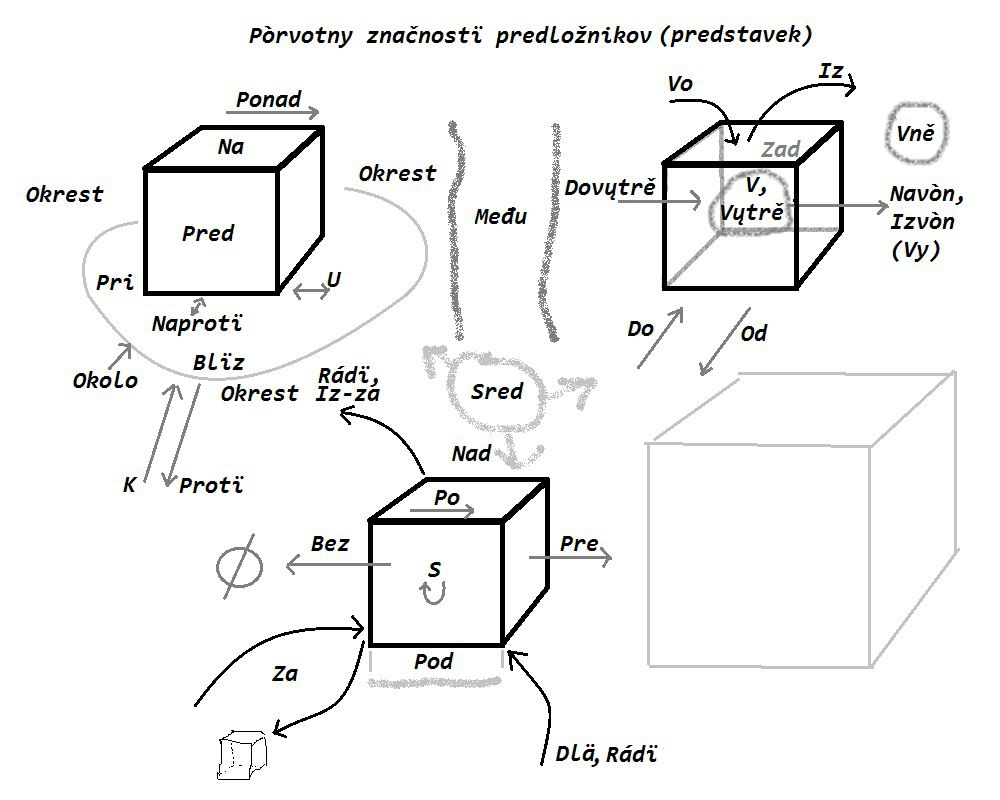
\includegraphics[width=\linewidth]{./sources/prepositions.jpeg}
	\caption{Prepositions in Novoslovnica}
	\label{fig:prepositions}
\end{figure}

Secondary prepositions are derived from nouns or adverbs with the shift of semantic from independent to an auxiliary one. For examples, preposition "Pred" is derived from the noun "Pred" (Front). Using separately in refers to a frontal part of something. Using with an additional independent word it becomes a preposition defining the frontal part of the word that follows it.

\textbf{Examples:}

\textit{Svòrh} - Over

\textit{Među} - Between
\section{Conjunction}

You see that there is a rather big amount of prepositions on Novoslovnica. However, the amount of conjunctions\index{conjunction} is much smaller. 

Conjunctions are divided into two classes: \textit{coordinating} and \textit{subordinating} conjunctions.

Coordinating\index{conjunction!coordinating} conjunctions usually connect sentence elements of the same grammatical class (N + N, V + V etc.). Syntactically, coordinating conjunctions connect either homogenuous sentense parts or independent clauses in a compound sentense. There are four kinds of coordinating conjunctions: copulative, adversative, disjunctive and illative.

\textbf{Conjunctive}:

I - and

Da - and

Ta - and

Ili - or

Či - or

Abo -or

\textbf{Adversative}:

Ale - but

Ama - but

No - but

Jednako - but

\textbf{Disjunctive}

Alïbo - either ... or

Lïbo - either ... or

A - and

\textbf{Illative}

Bo - because, that is why

Tako - thus, so

Subordinating\index{conjunction!subordinating} conjunctions are used to connect clauses in subordinate sentence. They complement the functionality of corresponding adverbs.

\textbf{Subordinative}:

Dabi - for

Aby - for

Da - for

This is the whole list of conjunctions existing in Novoslovnica today.

\section{Interjection}

This interesting POS is used to describe emotions within the sentence. Interjections\index{interjection} are neither independent nor dependent POS. They even are not involved into sentence structure. They just show the color of the sentence to let the interlocutor understand your feelings. 

Interjection is a POS that has no semantic meanings. Interjections are not words in our common comprehension. They are sounds that we produce. Sometimes it is rather difficult to say what differences are between interjections and senseless sounds that we can produce (i.e. some spontaneous exclaims, murmuring etc.). Interjections are divided into intended exclaims (with bright emotional color) and sound imitations (i.e. animal voices imitation) that are united in Novoslovnica within the POS of Onomatopoetics. So, Interjections in Novoslovnica are only used to express emotional exclaims.

Interjections are divided into three groups depending on their aim: emotional, imperative and etiquette. 

\textbf{Emotional interjections}

Emotional interjections can be divided into negative and positive interjections.

Positive:

Ah - Ah

Ŭaŭ - Wow

Ŭah - Wow

Ura - Hurray

Ogo - Wow

Uf - 

\textbf{Negative}

Oh - Oh

O-o - Oh

Be - 

Hehe -

Heh -  

Éh - 

Jo - 

Fu - 

\textbf{Ambiguous} (depend on the context):

Uh - Uh

Oǐ - Oh

Aǐ - 

Išty - 

Hm - Hmm

\textbf{Imperative interjections}

Let us look at them:

Éǐ - Hey

Na - Take it

Stop - Stop

Bre - Man

A-u - 

Allo - Hello

Brysj - Go out

Von - Out

\textbf{Etiquette interjections}

These interjections are often whole words, that we use without the sentence context in some situations that need our etiquette.

Hvála - Thanks

Dobrodošli - Welcome

Dękujem - Thanks

Zdråveǐ - Hi

Zdråveǐte - Hello

\section{Onomatopoetic words}


